% sudo apt update && sudo apt install -y texlive-full
% 使用 XeLaTeX 编译: xelatex thesis.min.tex
% CCF 中国计算机学会 A 类会议论文格式
% Swift: 启发式多信号融合自适应网络拥塞控制算法

\documentclass[10pt,twocolumn]{article}

% 中文支持
\usepackage[UTF8]{ctex}
\usepackage{fontspec}

% 数学公式
\usepackage{amsmath}
\usepackage{amssymb}

% 图表
\usepackage{graphicx}
\usepackage{float}
\usepackage{booktabs}
\usepackage{multirow}
\usepackage{array}

% 算法
\usepackage{algorithm}
\usepackage{algorithmic}

% 引用和链接
\usepackage{cite}
\usepackage{hyperref}
\usepackage{url}

% 颜色
\usepackage{xcolor}

% 页面设置
\usepackage{geometry}
\geometry{a4paper,left=1.9cm,right=1.9cm,top=2.2cm,bottom=2.2cm,columnsep=0.55cm}

% 行距
\usepackage{setspace}
\setstretch{1.08}

% 标题间距
\usepackage{titlesec}
\titlespacing*{\section}{0pt}{10pt}{5pt}
\titlespacing*{\subsection}{0pt}{7pt}{3pt}
\titlespacing*{\subsubsection}{0pt}{5pt}{2pt}
\titleformat{\section}{\normalfont\large\bfseries}{\thesection}{0.5em}{}
\titleformat{\subsection}{\normalfont\normalsize\bfseries}{\thesubsection}{0.5em}{}
\titleformat{\subsubsection}{\normalfont\small\bfseries}{\thesubsubsection}{0.5em}{}

% 紧凑列表
\usepackage{enumitem}
\setlist{nosep,leftmargin=1.2em}

% caption
\usepackage{caption}
\captionsetup{font=small,labelfont=bf,skip=4pt}

% 浮动体间距
\setlength{\textfloatsep}{8pt plus 2pt minus 2pt}
\setlength{\floatsep}{6pt plus 2pt minus 2pt}
\setlength{\intextsep}{6pt plus 2pt minus 2pt}
\setlength{\abovecaptionskip}{4pt}
\setlength{\belowcaptionskip}{2pt}

% 段落间距
\setlength{\parskip}{1.5pt plus 0.5pt minus 0.5pt}

% 算法环境字体
\usepackage{etoolbox}
\AtBeginEnvironment{algorithmic}{\small}

%% 英文字体默认使用 Times New Roman
\RequirePackage{xltxtra} % \XeTeX Logo
\setmainfont{Times New Roman}   % 衬线字体
\setsansfont{Arial}             % 无衬线字体
\setmonofont{Courier New}       % 等宽字体，一般是打印字体
%% 中文字体默认使用宋体
%\setCJKmainfont{songti}
\IfFontExistsTF{STXingkai}{
  \setCJKfamilyfont{hwxk}{STXingkai} % Windows
}{
  \setCJKfamilyfont{hwxk}{Sarasa Gothic SC} % Other
}
\newcommand{\stxk}{\CJKfamily{hwxk}}
\IfFontExistsTF{SimSun}{
  \setCJKfamilyfont{zhsong}[AutoFakeBold = {2.17}]{SimSun} % Windows
}{
  \setCJKfamilyfont{zhsong}[AutoFakeBold = {2.17}]{Sarasa Gothic SC} % Other
}
%\renewcommand{\songti}{\CJKfamily{zhsong}}

\begin{document}

%========================================
% 标题
%========================================

\title{\Large\textbf{Swift: 启发式多信号融合自适应网络拥塞控制算法}}

\author{
\normalsize 杭天铖 \\
\small 南京邮电大学 \\
\small 1224045520@njupt.edu.cn
}

\date{}

\maketitle

%========================================
% 摘要
%========================================

\begin{abstract}
\small
端到端网络传输的服务对象正在从固定终端和近端高质量链路，扩展到跨地域远距离传输、蜂窝/无线/卫星等多接入路径，以及手机、笔记本、台式机和边缘设备等异构终端并存的复杂场景。传统基于丢包的算法存在拥塞信号滞后与缓冲区膨胀问题，基于延迟的算法面临RTT测量噪声与共存公平性不足等缺陷；当长RTT、链路抖动与终端能力差异同时出现时，固定参数、单一信号驱动的拥塞控制更难兼顾吞吐、延迟与稳定性。本文提出Swift——一种面向远距离传输与异构终端的启发式多信号融合自适应拥塞控制方法，其核心创新收敛为三点：（1）\textbf{多信号拥塞状态感知}，将ECN协商与标记状态、拥塞避免状态机状态、拥塞事件语义、RTT与最小RTT、在途字节等协议栈内部信息组织为11维有效观测子空间（嵌入15元素状态传输容器，另含套接字标识、环境类型、仿真时间、节点标识四项跨进程路由元数据），并以两级优先级判定区分超时、ECN触发的窗口收缩与普通丢包；（2）\textbf{启发式反馈自适应的融合控制}，由最小RTT感知的RTT膨胀比、性能反馈值相对其自身慢速基线的偏移量以及连续增长趋势共同调节每流乘性增加因子$\alpha\in[0.85,1.30]$，并以有界步长逼近$\alpha\times BDP$目标窗口，其中BDP由滑动时间窗口投递速率的窗口最大值滤波给出；决策由协议栈外的确定性规则在每个确认事件上求解，不依赖训练样本与神经网络推理；（3）\textbf{面向不确定拥塞信号的稳定性与安全机制}，包括差异化窗口保留因子（丢包$\rho=0.70$、ECN $\rho=0.75$、超时$\rho=0.50$）、连续递减下限$D_{\max}=3$、降窗后4个ACK事件冻结、不迁就队列驻留的慢启动阈值更新以及窗口安全钳位。

在ns-3.40离散事件仿真平台上，本文以哑铃拓扑、3条并发长流评估Swift，实验矩阵覆盖36个场景（近端高速、共享汇聚、无线局域网、蜂窝接入、城域/跨域广域网与LEO/GEO卫星链路，瓶颈10 Mbps$\sim$100 Gbps、基线RTT 4 $\mu$s$\sim$640 ms），并在瓶颈上以\textbf{平均负载为瓶颈速率32\%、峰值速率64\%（50\%占空比）}的UDP突发流构成严格A/B对照，两种设置下共运行288次仿真。瓶颈队列统一采用启用ECN标记的RED（$MinTh=0.3Q$、$MaxTh=0.9Q$），并对四种协议对称开启ECN协商。全部指标仅按前向数据流定义（\texttt{logs/summary/kpi\_forward.csv}），288条记录全部通过物理相容性审计，无需排除任何场景。结果表明：纯TCP设置下Swift在\textbf{全部36个场景}取得最高聚合吞吐量，相对最强基线的增益为$+2.1\%\sim+5.8\%（均值+4.1\%）$，且该增益在微秒级近端链路、无线/蜂窝接入与远距离链路三类路径上均匀分布；平均单向时延相对NewReno/CUBIC均值低约2.3\%（36个场景中24个更低），与BBR基本相当；四协议丢包率全部不超过0.026\%，Jain公平性指数Swift均值0.9989为四者最高。UDP突发下Swift吞吐量保持率均值68.6\%（最差62.4\%），与基线持平，但\textbf{绝对吞吐量仍在全部36个场景领先}（相对最强基线$+2.2\%\sim+5.9\%$）；GEO卫星场景纯TCP吞吐量8.78 Mbps（相对NewReno $+7.5\%$）、突发下5.65 Mbps（相对NewReno $+10.1\%$）。本文同时如实披露混合结果：在\texttt{congested\_heavy}等深缓冲低速率场景及\texttt{wifi\_legacy}等链路上，Swift以约0.1$\sim$0.4 ms（相对值最高约10\%）的排队时延换取吞吐领先，且Swift的丢包率并不系统性低于基线（差值为0.001$\sim$0.003个百分点量级）。全部定量结果可在给定随机种子下逐项复现。

\vspace{0.3em}
\noindent\textbf{关键词：}拥塞控制；启发式自适应；多信号融合；显式拥塞通知；自适应参数调优；远距离传输；异构终端
\end{abstract}

%========================================
% 1. 引言
%========================================

\section{引言}

随着云计算、大数据、人工智能、移动互联网和物联网技术的蓬勃发展，端到端网络传输的服务对象正在从固定主机扩展到手机、笔记本、台式机、边缘节点和传感设备等异构终端，传输路径也从近端局域链路延伸到跨城、跨域、蜂窝接入、无线局域网和卫星通信等远距离复杂网络。TCP作为互联网传输层的核心协议，其拥塞控制机制的性能直接影响网络资源利用效率、应用响应延迟和用户体验。

在这类端到端传输场景中，网络路径和终端侧条件呈现出更强的异构性。一方面，城域/广域网、蜂窝网络、WiFi与卫星链路具有不同的RTT量级、丢包背景、可用带宽和链路抖动；另一方面，手机、电脑、边缘设备等终端在处理能力、无线接入方式、移动性和业务负载上差异显著。同一拥塞控制策略需要在短RTT近端高速链路与长RTT远距离链路之间切换，并在突发跨流量、无线误码和终端负载波动下保持稳定。上述复杂性使传统依赖固定参数或单一拥塞信号的算法难以同时满足高吞吐、低延迟和低丢包目标。

传统基于丢包的拥塞控制算法（如NewReno\cite{newreno}、CUBIC\cite{cubic}）将丢包作为拥塞信号，但丢包是拥塞的滞后指示器，通常意味着网络缓冲区已经溢出，排队延迟已累积到较高水平，产生"Bufferbloat"问题\cite{bufferbloat}。基于延迟的算法（如Vegas\cite{vegas}、BBR\cite{bbr}）尝试通过RTT变化提前感知拥塞，但RTT测量易受操作系统调度、路径抖动等因素干扰，且与基于丢包算法共存时存在严重的公平性问题\cite{bbrfairness}。

ECN机制\cite{rfc3168}允许网络设备在队列超过阈值时标记数据包而非丢弃，实现更早、更精确的拥塞通知。DCTCP\cite{dctcp}利用ECN标记比例进行细粒度调整，取得了良好效果。然而，现有算法对ECN信号的利用仍不够充分，大多采用静态参数配置，缺乏自适应能力。

近年来，强化学习在网络拥塞控制中的应用受到关注\cite{rlcc}。Aurora\cite{aurora}采用PPO算法训练深度神经网络策略，Orca\cite{orca}使用强化学习动态调整AIMD参数。然而，这类学习型方案通常需要离线训练与模型推理设施，状态空间设计不完善（通常仅4-6维）、未利用ECN和拥塞控制状态机信息、奖励函数难以平衡多目标、在训练分布之外泛化能力有限，且难以给出可审计的确定性行为。本文因此选择另一设计点：以协议栈内部信号驱动的\emph{白盒启发式规则}作为决策主体，仅在参数层引入轻量的反馈自适应，从而在保持$O(1)$决策开销与完全可复现性的同时获得跨场景的稳定性能。

与单一网络域相比，跨地域和多接入传输的拥塞信号更难解释。丢包可能来自真实队列溢出，也可能来自无线误码或链路切换；RTT升高既可能表示排队，也可能来自路径变化、终端调度延迟或接入链路抖动；突发UDP/RPC/视频/备份流量还会造成短时间带宽挤占。因此，Swift的设计目标不是某一类专用网络，而是端到端路径条件高度可变的通用传输场景。相应地，本文将微秒级RTT的近端高速链路、无线局域网、蜂窝接入、城域/跨域广域网与GEO卫星链路组织为一组覆盖不同RTT量级、带宽量级和接入条件的评估集合；其中短RTT高速率链路（如机架内与叶脊互联）仅作为该集合中RTT最小、排队延迟占比最高的一类\emph{被评估的网络条件}出现，并不构成算法的设计动机或部署前提。

针对上述挑战，本文提出Swift算法——一种启发式多信号融合自适应网络拥塞控制方法，其决策策略以每个ACK事件为粒度在协议栈之外以确定性规则求解，状态向量经同步请求—应答信道（ns-3侧由ns3-gym/OpenGym\cite{opengym}框架封装为15元素容器）在仿真进程与决策进程间传递。本文的核心创新收敛为如下三点：

\textbf{（1）面向远距离与异构终端的多信号拥塞状态感知}：将ECN协商与标记状态、拥塞避免状态机状态、拥塞事件语义、RTT与最小RTT、在途字节等协议栈内部信息组织为11维有效观测子空间，并据此以两级优先级判定区分超时、ECN触发的窗口收缩与普通丢包，为异构终端与多接入路径提供比"仅丢包"或"仅RTT"更完整的拥塞语义。

\textbf{（2）启发式反馈自适应的融合控制}：由最小RTT感知的RTT膨胀比、性能反馈值相对其自身慢速基线的偏移量以及连续增长趋势三路启发式信号共同调节每流乘性增加因子$\alpha \in [0.85, 1.30]$，并以有界步长逼近$\alpha \times BDP$目标窗口；BDP由滑动时间窗口投递速率的窗口最大值滤波给出，配合最小RTT自适应的HyStart风格慢启动退出与管道利用率感知加性递增，在吞吐、延迟与稳定性之间取得在线折中。

\textbf{（3）面向不确定拥塞信号的稳定性与安全机制}：依据信号严重程度施加差异化窗口保留因子（丢包0.70、ECN 0.75、超时0.50），并以连续递减下限$D_{\max}=3$、降窗后4个ACK事件冻结、不迁就队列驻留的慢启动阈值更新、窗口安全钳位以及超时时丢弃陈旧动作等机制，抑制误判信号与陈旧带宽估计导致的窗口过度收缩和振荡。

%========================================
% 2. 相关工作
%========================================

\section{相关工作}

\subsection{传统拥塞控制算法}

\subsubsection{基于丢包的算法}

TCP Tahoe和Reno是最早的拥塞控制算法\cite{jacobson1988}，引入了慢启动、拥塞避免和快速重传/恢复机制。TCP NewReno\cite{newreno}改进了快速恢复机制，能够处理突发丢包情况，是RFC 6582定义的标准算法。

TCP CUBIC\cite{cubic}是Linux自2.6.19版本以来的默认算法，采用三次函数模型调整窗口：
\begin{equation}
W(t) = C \cdot (t - K)^3 + W_{max}
\end{equation}
其中$K = \sqrt[3]{W_{max} \cdot \beta / C}$。CUBIC的窗口增长与RTT无关，在高BDP网络中具有更快的收敛速度。

基于丢包算法的共同缺陷包括：（1）拥塞信号滞后，缓冲区溢出前已积累大量排队延迟；（2）缓冲区膨胀，持续增加发送速率直至丢包；（3）无法区分拥塞程度，对所有拥塞采用统一的窗口减半策略。

\subsubsection{基于延迟的算法}

TCP Vegas\cite{vegas}通过比较期望吞吐量$cwnd/BaseRTT$与实际吞吐量$cwnd/RTT$的差值$\Delta$调整窗口，当$\Delta < \alpha$时增窗，$\Delta > \beta$时降窗。

BBR\cite{bbr}通过估计瓶颈带宽$BtlBw$和最小RTT $RTT_{prop}$，以BDP为目标调整发送速率：$pacing\_rate = pacing\_gain \times BtlBw$。BBR采用周期性增益调整实现带宽探测。

Copa\cite{copa}将目标排队延迟设为$RTT_{standing} - RTT_{min}$的函数，并引入竞争模式检测机制。

这类算法面临RTT测量不稳定（受调度延迟、路径抖动影响）、与丢包算法共存公平性差（研究表明BBR与CUBIC共存时吞吐量可下降30\%以上\cite{bbrfairness}）、参数敏感等问题。

\subsubsection{混合算法}

Compound TCP\cite{compound}叠加基于延迟的窗口分量，Illinois\cite{illinois}根据RTT调整AIMD参数，Westwood\cite{westwood}通过ACK到达率估计带宽。混合算法在一定程度上缓解了单一信号的局限性，但增加了复杂性。

\subsection{ECN机制与相关算法}

ECN\cite{rfc3168}通过IP报头中的2比特字段传递拥塞信息，定义四种码点（Non-ECT、ECT(0)、ECT(1)、CE）。发送端设置ECT标记表明支持ECN；网络设备在队列超阈值时将ECT改为CE；接收端回传ECE标志；发送端响应后设置CWR标志。

DCTCP\cite{dctcp}利用ECN标记比例$\alpha$进行细粒度调整：
\begin{equation}
\alpha = (1-g) \cdot \alpha + g \cdot F, \quad cwnd = cwnd \times (1 - \alpha/2)
\end{equation}
其中$g=1/16$是平滑因子，$F$是最近一个RTT内被标记的数据包比例。DCTCP能根据拥塞程度进行比例响应，但参数静态预设。HPCC\cite{hpcc}利用网络设备提供的INT精确拥塞信息进行控制，但需要特殊硬件支持。

ECN的优势在于：（1）在丢包前提供明确拥塞信号；（2）避免重传开销；（3）信号来自网络设备显式标记，比RTT推测更可靠。然而，现有算法对ECN的利用仍不充分。

\subsection{基于强化学习的拥塞控制}

Aurora\cite{aurora}采用PPO算法训练神经网络策略，使用10维状态空间（延迟梯度、延迟比率、发送比率等），奖励函数为$r = throughput - \delta \cdot delay - \lambda \cdot loss$。Orca\cite{orca}在AIMD框架下用强化学习动态调整增加因子$\alpha$和减少因子$\beta$。PCC\cite{pcc}定义实用函数$U(x) = T \cdot x^\alpha - \delta \cdot L \cdot x - \beta \cdot D \cdot x$，通过梯度上升最大化。Remy\cite{remy}采用离线优化生成规则。

现有方法的共同问题是：（1）状态空间较窄，通常为4$\sim$6维，未利用ECN和CA状态等协议栈内部信息；（2）奖励函数设计困难，多目标权衡复杂；（3）训练与再训练成本高、推理依赖重；（4）在训练分布之外的路径条件上泛化能力有限。Swift因此不采用学习型策略，而是在状态表示上引入协议栈内部信号，以\emph{确定性启发式规则}完成全部窗口决策，仅在参数层使用基线相对的反馈自适应；本文不主张Swift在表示能力上优于深度策略，二者的取舍差异见第\ref{sec:discussion}节。

\subsection{参数化白盒控制与带外参数优化}
\label{subsec:gemini}

与"用学习模型替换控制逻辑"不同，另一类工作把学习限制在\emph{参数}层面。Gemini\cite{gemini}采用分而治之框架：其参数化拥塞控制类Fusion以Linux内核模块形式实现固定的白盒控制逻辑（融合窗口式与速率式增长，以丢包率阈值$l$和RTT膨胀阈值$\delta$作为拥塞信号，并以$\alpha \cdot R^{\max}T^{\min}$为窗口目标），其在线优化引擎Booster则运行在用户态集群中，按分钟级时间窗口聚合流级统计量，并用贝叶斯优化在隐变量（区域、ISP、时段）分组内搜索控制参数$\theta=\{\omega,\alpha,\gamma,\lambda,l,\delta,n\}$。该设计的优势是数据面开销与传统算法相当，且已在生产网络完成大规模部署验证。

Swift与之处于不同的设计点。第一，\textbf{决策位置与时间尺度}：Gemini的控制逻辑固定在内核数据面内，学习（贝叶斯优化）只在带外、以分钟级和流组粒度更新参数；Swift把整个决策策略置于协议栈之外，并在每个ACK事件（GetSsThresh/IncreaseWindow回调）上被同步调用，因此其自适应发生在单流、单事件粒度上。第二，\textbf{可用信号}：带外优化器只能观察流级统计量，而Swift的状态向量直接来自协议栈内部，可读取ECN状态机与拥塞避免状态机，从而区分ECE/CWR触发的收缩与真实丢包。第三，\textbf{部署代价}：这一选择的代价是每事件一次跨进程往返，本文实现依赖ZeroMQ同步通信，在当前形态下适用于仿真与研究平台，而非生产数据面；Gemini的内核态Fusion在这一维度上明显更易部署。第四，\textbf{证据强度}：Gemini给出了生产网络A/B测试结果，本文的证据仅来自ns-3.40仿真。因此，本文将Swift定位为“协议栈外每事件启发式决策 + 协议栈内多信号感知”这一设计点的可行性与代价评估，而非对Gemini式部署路线的替代。

%========================================
% 3. Swift算法设计
%========================================

\section{Swift算法设计}

\subsection{系统架构}

Swift的系统架构由四个核心模块组成，整体控制回路如图\ref{fig:architecture}所示。\textbf{网络仿真模块}基于ns-3\cite{ns3}构建，实现完整TCP/IP协议栈和多种网络拓扑（近端高速链路、哑铃型、无线/移动、广域网与卫星链路等）。\textbf{状态采集与决策应用模块}在TCP协议栈的五个关键回调点（GetSsThresh、IncreaseWindow、PktsAcked、CongestionStateSet、CwndEvent）采集11维状态参数，并将决策模块输出的ssthresh/cwnd决策应用于TCP连接（该模块基于ns3-gym/OpenGym\cite{opengym}环境框架实现，仅作为跨进程状态—决策传输通道，不含任何学习逻辑）。\textbf{启发式决策模块}采用Python实现，执行多信号融合拥塞检测、差异化拥塞响应、自适应参数调优和融合控制策略计算，维护每个TCP连接的独立状态。\textbf{进程间通信模块}采用ZeroMQ消息队列和Protocol Buffers序列化，实现仿真进程与决策进程间的同步请求—应答交互；由于该路径依赖ZMQ同步通信，当前实验未启用MTP并行仿真。

\begin{figure*}[!t]
\centering
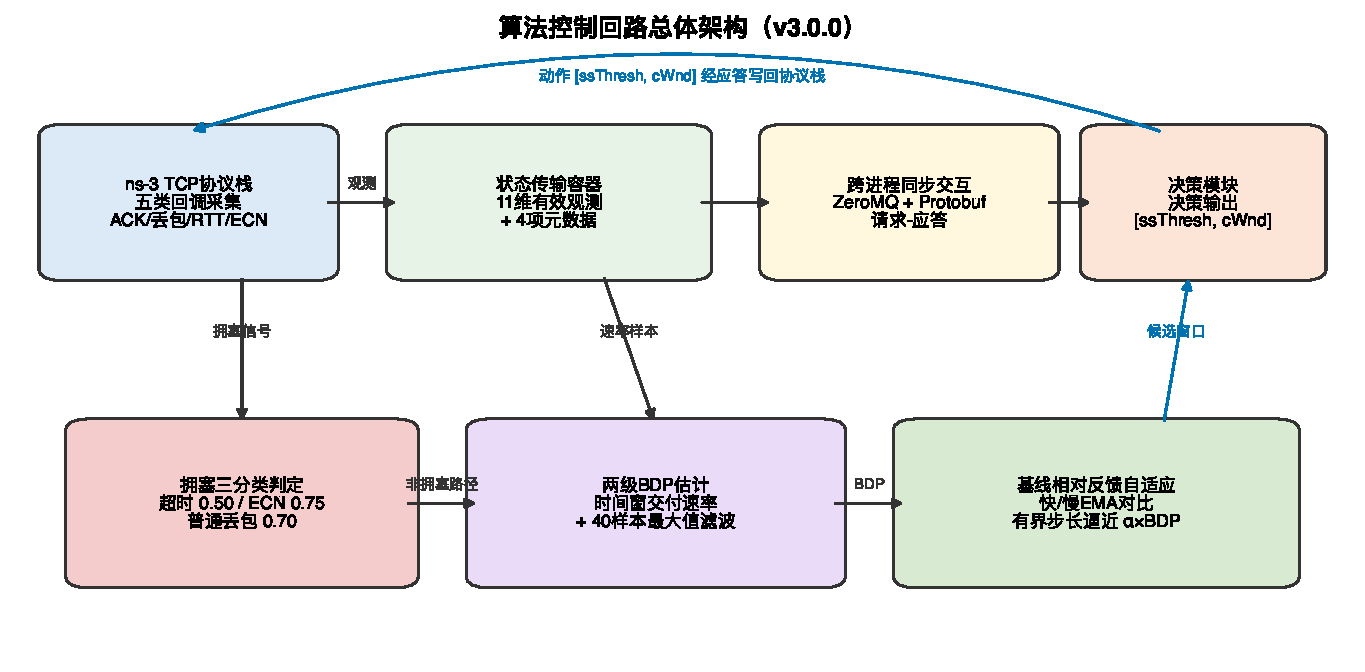
\includegraphics[width=0.86\textwidth]{plots/fig06_architecture_zh.pdf}
\caption{Swift控制回路总体架构：协议栈回调采集的状态向量经跨进程同步信道送入启发式决策模块，依次执行拥塞三分类判定、两级BDP估计与基线相对反馈自适应，ssthresh/cwnd决策经应答写回协议栈}
\label{fig:architecture}
\end{figure*}

Swift的决策问题可描述为一个\emph{每事件决策回路}：在每个窗口调整回调上，以当前状态向量$s$（11维有效状态，嵌入于15元素传输容器，另含4项元数据通道）为输入，由确定性规则直接输出新的ssthresh和cwnd决策值$\langle ssthresh, cwnd \rangle$。该表示以“状态—决策—反馈”三元组刻画：性能反馈值$r_t$由环境按确认进度与排队/丢包代价合成，仅用于参数层的慢速自适应（见第\ref{subsubsec:alpha}节），不构成任何策略学习信号。

状态向量设计满足以下原则：（1）\textbf{信息充分性}——11维空间涵盖TCP协议栈所有关键信息（ECN状态、CA状态、窗口与RTT），避免因信息不足导致的次优决策；（2）\textbf{可观测性}——所有参数均可从ns-3标准回调接口直接获取；（3）\textbf{维度可控性}——11维状态处理与规则决策的时间复杂度均为$O(1)$，不存在高维表示导致的维度灾难问题。

\subsection{11维观测空间设计}

Swift的状态向量采用“11维有效状态子空间 + 4项元数据通道”的15元素传输布局，如表\ref{tab:observation}所示。参数涵盖六大类别:连接标识(socketUuid、nodeId)用于多流识别和状态隔离;时间信息(envType、simTime)用于时序分析和投递速率计算;窗口状态(ssthresh、cwnd)是拥塞控制的核心变量;传输性能(segSize、segmentsAcked、bytesInFlight)用于吞吐量估算和管道利用率计算;延迟测量(lastRtt、minRtt)用于BDP估算和拥塞程度判断;回调类型与拥塞控制状态(calledFunc、caState、caEvent、ecnState)提供协议栈完整状态。其中前4项（socketUuid、envType、simTime、nodeId）为跨进程路由用的元数据，不参与窗口决策；后11项构成参与AIMD/ECN响应/$\alpha$自适应的有效状态，故本文后续统称“11维观测”指该有效子空间。

\begin{table}[htbp]
\centering
\caption{Swift 11维有效观测子空间（对应15元素容器索引4$\sim$14）}
\label{tab:observation}
\small
\begin{tabular}{clp{3.2cm}}
\toprule
\textbf{索引} & \textbf{参数} & \textbf{说明} \\
\midrule
4  & ssThresh & 慢启动阈值(B) \\
5  & cwnd & 拥塞窗口(B) \\
6  & segSize & 段大小(B) \\
7  & segmentsAcked & 确认段数 \\
8  & bytesInFlight & 在途字节数 \\
9  & lastRtt & 最近RTT($\mu$s) \\
10 & minRtt & 最小RTT($\mu$s) \\
11 & calledFunc & 回调类型(0/1) \\
12 & caState & CA状态(0-4) \\
13 & caEvent & CA事件(0-5) \\
14 & ecnState & ECN状态(0-5) \\
\bottomrule
\end{tabular}
\end{table}

Swift的核心创新在于引入三个协议栈内部状态参数。\textbf{caState}反映TCP拥塞控制状态机的当前状态：CA\_OPEN（0，正常传输）、CA\_DISORDER（1，收到重复确认）、CA\_CWR（2，响应ECN缩减窗口）、CA\_RECOVERY（3，快速恢复中）、CA\_LOSS（4，超时丢包）。\textbf{caEvent}表示最近的拥塞事件：包括CA\_EVENT\_TX\_START（0）、CWND\_RESTART（1）、COMPLETE\_CWR（2）、LOSS（3）、ECN\_NO\_CE（4）、ECN\_IS\_CE（5）六种。\textbf{ecnState}反映ECN协商和标记状态：ECN\_DISABLED（0）、ECN\_IDLE（1）、ECN\_CE\_RCVD（2）、ECN\_SENDING\_ECE（3）、ECN\_ECE\_RCVD（4）、ECN\_CWR\_SENT（5）。

这三个参数的引入使决策模块能够感知TCP协议栈的完整状态信息，从而把协议栈内部语义纳入每事件决策。所有15个参数均可从ns-3 TCP模块的标准回调接口直接获取，满足可观测性要求。11维有效状态的处理时间复杂度为$O(1)$，无任何神经网络推理依赖。

\subsection{多信号融合拥塞检测}

Swift将拥塞信号分为三类，采用两级优先级层次结构进行综合判断，并引入连续递减保护机制防止窗口过度收缩。

\textbf{第一优先级——窗口收缩回调检测}：当$calledFunc = 0$时（GetSsThresh回调），表明协议栈正在执行窗口收缩。此时进一步区分收缩原因：若$caState = \text{CA\_LOSS}$，判定为超时丢包（通常意味着连续多个数据包丢失或网络路径中断）；若$ecnState \in \{\text{ECN\_CE\_RCVD}, \text{ECN\_ECE\_RCVD}\}$或$caState = \text{CA\_CWR}$，说明本次收缩由ECN回显（ECE）触发，判定为ECN标记并施加ECN保留因子；否则判定为普通丢包（快速重传触发）。丢包和超时是最可靠的拥塞信号（似然比$LR \approx 100$），一旦检测到即触发响应。

\textbf{第二优先级--ECN状态直接检测}:当$ecnState \in \{\text{ECN\_CE\_RCVD}, \text{ECN\_ECE\_RCVD}\}$时,判定存在ECN拥塞标记。与基于事件率统计的方法不同,Swift直接检查协议栈的ECN状态字段,避免了维护时间戳队列的额外开销和事件率阈值的参数敏感性问题。需要强调的是，该分支成立的前提是瓶颈队列管理器确实执行CE标记：若瓶颈使用不标记CE的先进先出队列，则$ecnState$不会进入CE/ECE状态，ECN分支恒不触发。第\ref{subsec:setup}节据此将瓶颈默认配置为启用ECN标记的RED队列，并对全部对比协议对称开启ECN；本文所引用的实验产物即在该配置下生成。

\textbf{连续递减保护机制}：为防止在突发拥塞期间窗口被过度收缩，Swift维护一个连续递减计数器$d$。每次触发拥塞响应时$d$自增；仅当窗口真正发生增长时$d$才被重置为零——在降窗后的冻结期内窗口保持不变，因此$d$不被清零，从而使保护逻辑对连续到达的拥塞信号保持记忆。当$d$超过最大连续递减次数$D_{max} = 3$时，拥塞响应被抑制——保持当前窗口不变，避免因连续乘性递减导致窗口收缩至过小值。连续3次丢包响应后窗口仅剩$0.70^3 \approx 34.3\%$，已强于传统算法单次窗口减半的效果，进一步缩减的边际收益递减。

完整的多信号融合拥塞检测算法如算法\ref{alg:detect}所示。

\begin{algorithm}[htbp]
\caption{Multi-Signal Fusion Congestion Detection}
\label{alg:detect}
\small
\begin{algorithmic}[1]
\REQUIRE Observation $obs$, consecutive decrease counter $d$
\ENSURE $(is\_congested, \; type)$
\STATE \textbf{// Level-1: window-reduction callback (GetSsThresh)}
\IF{$obs.calledFunc = 0$}
    \IF{$obs.caState = \text{CA\_LOSS}$}
        \RETURN $(True, \; \text{TIMEOUT})$
    \ELSIF{$obs.ecnState \in \{\text{CE\_RCVD}, \text{ECE\_RCVD}\}$ \textbf{or} $obs.caState = \text{CA\_CWR}$}
        \RETURN $(True, \; \text{ECN})$
    \ELSE
        \RETURN $(True, \; \text{LOSS})$
    \ENDIF
\ENDIF
\STATE \textbf{// Level-2: ECN state inspection}
\IF{$obs.ecnState \in \{\text{CE\_RCVD}, \text{ECE\_RCVD}\}$}
    \RETURN $(True, \; \text{ECN})$
\ENDIF
\RETURN $(False, \; \text{NONE})$
\end{algorithmic}
\end{algorithm}

\subsection{差异化拥塞响应机制}

传统算法（如NewReno、CUBIC）对所有拥塞信号采用统一的窗口减半策略（保留因子$\rho=0.5$），这种"一刀切"的方法无法区分轻度和严重拥塞，在轻度拥塞时响应过度（不必要地降低吞吐量），在严重拥塞时响应不足。Swift根据拥塞类型设计差异化的窗口保留因子：

\begin{equation}
\begin{aligned}
new\_cwnd &= \rho \cdot cwnd, \\
\rho &= \begin{cases}
0.70 & \text{丢包(LOSS)} \\
0.75 & \text{ECN标记} \\
0.50 & \text{超时(TIMEOUT)}
\end{cases}
\end{aligned}
\end{equation}

设计依据如下。（1）\textbf{拥塞信号的时序特性}：ECN标记是最早的信号（队列超低阈值时触发），丢包较晚（队列溢出），超时最晚（连续丢包或路径问题）。早期信号应采用相对温和但足以排空队列的响应，晚期信号采用更激进的响应。（2）\textbf{信号可靠性}：丢包几乎不会误报（$LR \approx 100$），ECN的可靠性取决于设备配置，因此对丢包响应更坚决。（3）\textbf{吞吐量-延迟权衡}：丢包保留因子0.70高于传统的0.5，配合ECN的提前预警机制实现更平滑的响应；当前实现将ECN保留因子设为0.75，使早期拥塞预警能够触发25\%的窗口收缩，以降低持续排队驻留风险；超时保留因子0.50与传统窗口减半一致，反映超时信号所指示的严重拥塞或路径故障。

慢启动阈值更新为$new\_ssthresh = \max(\rho \cdot \min(cwnd, BDP), \; new\_cwnd)$：以$\min(cwnd, BDP)$为基准可避免将阈值抬升至BDP以上而变相鼓励队列驻留，同时以$new\_cwnd$为下界保证拥塞避免阶段仍可缓慢上探。窗口下限约束为$4 \times MSS$。

此外，当前实现在拥塞响应路径上还包含三项与信号不确定性直接相关的安全约束。（1）\textbf{降窗后冻结}：每次进入拥塞响应即将冻结计数器置为4个ACK事件，且该赋值先于连续递减下限判定执行，因此即使响应被$D_{max}$抑制，队列仍获得排空窗口。（2）\textbf{超时重入慢启动}：当拥塞类型为超时时，除施加$\rho=0.50$外还重置慢启动标志与慢启动阶段最小RTT采样，使控制律回到指数上探而非在错误的BDP估计附近继续微调。（3）\textbf{陈旧动作丢弃}：由于GetSsThresh回调接收的是常量协议栈状态，Python侧返回的$cwnd$需缓存至下一次IncreaseWindow才能生效；若在此期间协议栈进入CA\_LOSS（重传超时已重置窗口），环境侧将直接丢弃该缓存动作，避免陈旧决策覆盖协议栈的丢包恢复过程。差异化响应算法如算法\ref{alg:response}所示。

\begin{algorithm}[htbp]
\caption{Differentiated Congestion Response}
\label{alg:response}
\small
\begin{algorithmic}[1]
\REQUIRE Current $cwnd$, congestion type $type$, consecutive decrease counter $d$, BDP estimate $bdp$
\ENSURE New window $new\_cwnd$, new threshold $new\_ssthresh$
\STATE $d \leftarrow d + 1$; \; consecutive increases $\leftarrow 0$
\STATE $freeze \leftarrow 4$ \COMMENT{Post-decrease freeze, armed before the floor test}
\IF{$d > D_{max}$}
    \STATE $new\_cwnd \leftarrow \max(cwnd, \; 4 \times MSS)$ \COMMENT{Freeze window}
    \STATE $new\_ssthresh \leftarrow new\_cwnd$
    \RETURN $(new\_cwnd, \; new\_ssthresh)$
\ENDIF
\IF{$type = \text{LOSS}$}
    \STATE $\rho \leftarrow 0.70$
\ELSIF{$type = \text{ECN}$}
    \STATE $\rho \leftarrow 0.75$
\ELSIF{$type = \text{TIMEOUT}$}
    \STATE $\rho \leftarrow 0.50$; \; re-enter slow start
\ENDIF
\STATE $new\_cwnd \leftarrow \max(\rho \times cwnd, \; 4 \times MSS)$
\STATE $new\_ssthresh \leftarrow \max(\rho \times \min(cwnd, \; bdp), \; new\_cwnd)$
\RETURN $(new\_cwnd, \; new\_ssthresh)$
\end{algorithmic}
\end{algorithm}

\subsection{启发式反馈自适应的参数调优}
\label{subsubsec:alpha}

Swift根据多种网络状态因素动态调整乘性增加因子$\alpha \in [0.85, 1.30]$（初始值1.10），控制拥塞避免阶段窗口增长速度。当前实现的调优逻辑基于RTT膨胀、反馈值EMA和连续增长趋势三个启发式维度。与固定阈值不同，RTT膨胀阈值会随最小RTT增大而放宽，使长RTT路径不会因为正常的BDP填充过程过早触发收缩。

\textbf{基于最小RTT感知阈值的调整}：设$r = lastRtt/minRtt$。Swift首先根据$minRtt$计算松弛量$slack = 0.3 + 0.15\sqrt{\max(0,minRtt_{ms}-1)}$，并构造$low=1+slack$、$mid=1+2slack$、$high=1+4slack$三个动态阈值。当$r < low$时，说明队列驻留较低，$\alpha$按0.02或0.03小步增加；当$low \leq r < mid$时，$\alpha$仅增加0.01以维持温和探测；当$r > high$时，说明排队膨胀明显，$\alpha$按0.02或0.03收缩并重置连续增长计数器。

\textbf{基于反馈值基线相对比较的调整}：为捕获较长期性能趋势，同时维护性能反馈值（由环境按确认进度与排队/丢包代价合成，记$r_t$）的快速指数移动平均$\bar{r}_t = (1 - \eta) \cdot \bar{r}_{t-1} + \eta \cdot r_t$（$\eta=0.15$）与慢速基线$b_t = (1 - \eta_b) \cdot b_{t-1} + \eta_b \cdot r_t$（$\eta_b=0.02$）。由于逐ACK反馈值几乎恒为正（每个确认段贡献$+0.5$的吞吐收益），固定绝对阈值不携带调节信息；因此仅当$\bar{r} > b + m$时$\alpha \mathrel{+}=0.01$，当$\bar{r} < b - 4m$时$\alpha \mathrel{-}=0.01$，其中动态裕量$m = \max(0.25, 0.1|b|)$，非对称下界使丢包/超时的惩罚尖峰仍能迅速收缩$\alpha$。环境侧的反馈值在ACK事件上定义为$r = \min(0.5\,segmentsAcked, 5) - p_{rtt}$，其中仅当$lastRtt/RTT_{min}>1.5$时$p_{rtt}=\min(0.3(lastRtt/RTT_{min}-1.5), 3)$，否则为零；在窗口收缩回调上则给出固定惩罚：ECN为$-3$、超时（CA\_LOSS）为$-20$、其他丢包为$-10$。由此反馈值同时携带传输进度与排队/丢包代价信息，而其绝对量级不影响$\alpha$调节——只有相对基线的变化量被使用。

\textbf{基于连续增长趋势的调整}：窗口连续增长超过8次时，说明当前路径仍具备可探测空间，$\alpha \mathrel{+}=0.01$。所有调整均限制在$[0.85,1.30]$内，以避免无线、蜂窝和广域网场景中的持续队列堆积。完整的$\alpha$自适应过程如算法\ref{alg:adapt}所示。

\begin{algorithm}[htbp]
\caption{RTT- and Reward-Aware Adaptive Parameter Tuning}
\label{alg:adapt}
\small
\begin{algorithmic}[1]
\REQUIRE Current $\alpha$, observation $obs$, consecutive increase count $g$, reward EMA $\bar{r}$, reward baseline $b$
\ENSURE Updated $\alpha$
\STATE $r \leftarrow obs.lastRtt \;/\; obs.minRtt$
\STATE $slack \leftarrow 0.3 + 0.15\sqrt{\max(0, obs.minRtt_{ms}-1)}$
\STATE $low \leftarrow 1+slack$; $mid \leftarrow 1+2slack$; $high \leftarrow 1+4slack$
\IF{$r < low$}
    \STATE $\alpha \leftarrow \alpha + (obs.minRtt_{ms}>5 ? 0.02 : 0.03)$; $g \leftarrow g+1$
\ELSIF{$r < mid$}
    \STATE $\alpha \leftarrow \alpha + 0.01$
\ELSIF{$r > high$}
    \STATE $\alpha \leftarrow \alpha - (obs.minRtt_{ms}>5 ? 0.03 : 0.02)$; $g \leftarrow 0$
\ENDIF
\STATE $m \leftarrow \max(0.25, \; 0.1\,|b|)$
\IF{$\bar{r} > b + m$}
    \STATE $\alpha \leftarrow \alpha + 0.01$
\ELSIF{$\bar{r} < b - 4m$}
    \STATE $\alpha \leftarrow \alpha - 0.01$
\ENDIF
\IF{$g > 8$}
    \STATE $\alpha \leftarrow \alpha + 0.01$
\ENDIF
\STATE $\alpha \leftarrow \text{clamp}(\alpha, \; 0.85, \; 1.30)$
\end{algorithmic}
\end{algorithm}

\subsection{融合控制策略}

Swift将BDP估计、目标窗口渐进逼近和安全边界约束相结合。BDP估计采用窗口最大值滤波器（Windowed Max-Filter）：投递速率由滑动时间窗口内的累计确认字节数计算，$DR = \Delta bytes_{acked} / \Delta t$，时间窗口跨度取$\min(\max(2 \times RTT_{min}, 5\,\text{ms}), 1\,\text{s})$，使速率反映ACK时钟（即瓶颈排空速率）而非单个ACK的载荷（后者会按每RTT的ACK数量成倍低估带宽）；速率样本存入容量为$W_{bw}=40$的滑动窗口队列，取窗口内最大值$BW_{max}$作为瓶颈带宽估计；RTT采样窗口容量为$W_{rtt}=40$，并持续跟踪全局最小RTT。BDP计算为$BDP = BW_{max} \times RTT_{min}$；当BDP估计无效时回退至当前窗口值。BDP估计算法如算法\ref{alg:bdp}所示。

\begin{algorithm}[htbp]
\caption{Windowed Max-Filter BDP Estimation}
\label{alg:bdp}
\small
\begin{algorithmic}[1]
\REQUIRE Flow state $state$, observation $obs$
\ENSURE BDP estimate
\STATE $state.bytes_{acked} \leftarrow state.bytes_{acked} + obs.segAcked \times obs.segSize$
\STATE $W \leftarrow \min(\max(2 \times RTT_{min}, \; 5\,\text{ms}), \; 1\,\text{s})$ \COMMENT{Rate window span}
\STATE $dr \leftarrow \Delta bytes_{acked} \;/\; \Delta t$ over the last $W$ \COMMENT{Delivery rate}
\STATE $state.bw\_samples$.append($dr$) \COMMENT{Sliding window, capacity $W_{bw}=40$}
\STATE $BW_{max} \leftarrow \max(state.bw\_samples)$
\STATE $RTT_{min} \leftarrow \min(state.min\_rtt, \; obs.minRtt)$
\STATE $bdp \leftarrow BW_{max} \times RTT_{min}$
\IF{$bdp \leq 0$}
    \STATE $bdp \leftarrow \max(obs.cwnd, \; 1)$ \COMMENT{Fallback}
\ENDIF
\RETURN $bdp$
\end{algorithmic}
\end{algorithm}

\textbf{慢启动阶段}（$cwnd < ssthresh$）：目标窗口$target = 2 \times BDP$（下限$10 \times MSS$）。Swift采用HyStart风格慢启动退出：当当前RTT超过慢启动阶段最小RTT的动态阈值时，提前退出慢启动以避免首轮BDP填充后的突发排队；该阈值随最小RTT从1.25放宽到1.40，使广域网和卫星链路不因正常长RTT特性过早退出。标准增量为$segmentsAcked \times MSS$；仅当当前窗口明显低于BDP且RTT尚未膨胀时，增量才提升为$2 \times segmentsAcked \times MSS$。

\textbf{拥塞避免阶段}（$cwnd \geq ssthresh$）：当前实现先计算目标速率窗口$target=\alpha \times BDP$（BDP无效时回退到当前窗口），再以有界步长向目标靠拢，而不是直接把窗口跳变到目标值。当$target>cwnd$时，窗口按$\max(\gamma\times MSS, MSS, (target-cwnd)/16)$上探，并以$target+\gamma\times MSS$为本次上限，从而在约16个ACK事件内完成BDP填充而不产生超调；当$target<cwnd$时，每个ACK事件按$\max((cwnd-target)/2, MSS)$回落且不低于$target$，以主动排空队列；当二者相等时，按$\gamma\times MSS$进行Reno式加性增长。当前实现取$\gamma=1.0$。此外，若降窗冻结计数器非零，本次事件直接返回当前窗口并将计数器减一，冻结期内不做任何增长。

\textbf{管道利用率感知加速与安全边界}：管道利用率$u = bytesInFlight/cwnd$用于识别未充分填充的链路。该增量仅在RTT未明显膨胀（$lastRtt < 1.3\,RTT_{min}$）时生效：当$u<0.4$时，短RTT路径追加$2\times MSS$，最小RTT超过5 ms的长RTT路径仅追加$1\times MSS$；当$0.4 \leq u<0.5$时，只有短RTT路径再追加$1\times MSS$。这一分级设计避免了在无线、蜂窝和广域网场景中因盲目加速而累积队列。最终窗口被约束在$[4\times MSS, \max(4\times BDP, 200\times MSS)]$内，避免BDP估计陈旧时窗口失控。融合控制策略的完整算法如算法\ref{alg:fusion}所示。

\begin{algorithm}[htbp]
\caption{Hybrid Rate-Window Fusion Control}
\label{alg:fusion}
\small
\begin{algorithmic}[1]
\REQUIRE Observation $obs$, parameter $\alpha$, BDP estimate $bdp$, freeze counter $f$
\ENSURE New window $new\_cwnd$
\IF{$f > 0$}
    \STATE $f \leftarrow f - 1$; \; \RETURN $obs.cwnd$ \COMMENT{Post-decrease freeze}
\ENDIF
\STATE $d \leftarrow 0$ \COMMENT{Reset the consecutive-decrease counter only on growth}
\IF{$obs.cwnd < obs.ssthresh$ and flow is in slow start}
    \STATE Apply HyStart-style RTT-inflation exit ($1.25/1.30/1.40$ by $RTT_{min}$)
    \STATE $target \leftarrow \max(2 \times bdp, \; 10 \times MSS)$
    \STATE $\Delta \leftarrow obs.segmentsAcked \times MSS$
    \IF{$obs.cwnd < 0.3 \times bdp$ and $obs.lastRtt < 1.2\,RTT_{min}$}
        \STATE $\Delta \leftarrow 2 \times obs.segmentsAcked \times MSS$
    \ENDIF
    \STATE $new\_cwnd \leftarrow \min(obs.cwnd + \Delta, \; target)$
\ELSE
    \STATE $target \leftarrow \alpha \times bdp$
    \IF{$target > obs.cwnd$}
        \STATE $step \leftarrow \max(\gamma \times MSS, \; MSS, \; (target-obs.cwnd)/16)$
        \STATE $new\_cwnd \leftarrow \min(obs.cwnd + step, \; target + \gamma \times MSS)$
    \ELSIF{$target < obs.cwnd$}
        \STATE $new\_cwnd \leftarrow \max(obs.cwnd - \max(\tfrac{obs.cwnd-target}{2}, MSS), \; target)$
    \ELSE
        \STATE $new\_cwnd \leftarrow obs.cwnd + \gamma \times MSS$
    \ENDIF
\ENDIF
\IF{$obs.lastRtt < 1.3\,RTT_{min}$}
    \STATE $u \leftarrow obs.bytesInFlight / obs.cwnd$
    \IF{$u < 0.4$}
        \STATE $new\_cwnd \leftarrow new\_cwnd + (RTT_{min} > 5\,\text{ms} \; ? \; MSS : 2 \times MSS)$
    \ELSIF{$u < 0.5$ \textbf{and} $RTT_{min} \leq 5\,\text{ms}$}
        \STATE $new\_cwnd \leftarrow new\_cwnd + MSS$
    \ENDIF
\ENDIF
\STATE $new\_cwnd \leftarrow \text{clamp}(new\_cwnd, \; 4 \times MSS, \; \max(4 \times bdp, \; 200 \times MSS))$
\RETURN $new\_cwnd$
\end{algorithmic}
\end{algorithm}

\subsection{每流独立状态管理}

Swift为每个TCP连接维护独立状态，通过socketUuid为键的哈希表实现$O(1)$查找。每流状态包括四个子模块：（1）\textbf{带宽与RTT估计模块}——容量$W_{bw}=40$的投递速率滑动窗口队列和容量$W_{rtt}=40$的RTT采样队列，支持窗口最大值带宽估计、全局最小RTT追踪和慢启动阶段最小RTT采样；（2）\textbf{拥塞控制计数器}——连续递减计数器$d$、连续增长计数器$g$、累计丢包和ECN事件计数，以及降窗后的ACK冻结计数；（3）\textbf{性能指标聚合}——吞吐量指数移动平均、当前BDP估计、上一步窗口和时间戳；（4）\textbf{自适应参数}——$\alpha$（初始1.10）、$\gamma$（默认1.0）和慢启动标志位。

状态管理遵循延迟初始化（首次访问时创建）和增量更新（仅更新变化字段）两个原则。每流独立管理避免了多流并发场景下的流间干扰，支持差异化控制。反馈值EMA（平滑因子$\eta=0.15$）与慢速基线（$\eta_b=0.02$）由每个连接对应的决策实例独立维护，避免流间反馈串扰。

%========================================
% 4. 实验评估
%========================================

\section{实验评估}

\subsection{仿真配置与实验矩阵}
\label{subsec:setup}

\textbf{软硬件环境}：ns-3.40\cite{ns3}与ns3-gym\cite{opengym}，Python 3.8，Intel i7-10700K（8核）处理器、32 GB内存、Ubuntu 20.04。

\textbf{拓扑与负载}：使用\texttt{PointToPointDumbbellHelper}构造哑铃拓扑，左右各3个叶子节点（$nLeaf=3$）经接入链路汇聚到一条共享瓶颈链路；每对叶子节点上运行一条\texttt{BulkSendHelper}长流，3条流分别在0、100与200 ms错峰启动，仿真时长20 s。MTU取1500 B，应用数据单元（MSS）为1440 B，启用SACK；瓶颈队列长度按$\max(BDP \cdot nLeaf / MTU, \; 100)$个报文配置，其中$BDP$由瓶颈速率与基础RTT算出，使缓冲深度随场景带宽和时延同步伸缩。

\textbf{队列管理与ECN}：瓶颈两侧网关统一安装RED队列，标记下限$MinTh = 0.3Q$、上限$MaxTh = 0.9Q$、\texttt{UseEcn=true}，并对四种协议一律设置\texttt{TcpSocketBase::UseEcn=On}，使ECN早期预警信号在对照协议之间对称可得。本文引用的全部实验产物（\path{logs/comparison/}与\path{logs/comparison-udp/}，2026-09-09批量运行）均在该配置下、由时间窗口投递速率估计与基线相对反馈自适应的当前实现（v3.0.0）生成，因此ECN分支、对称ECN与修正后的带宽估计器均为真实可观测的配置项，不再存在“ECN仅对Swift开启”或“队列不置CE”之类的历史不对称。

\textbf{A/B对照设置}：两组实验共享完全相同的场景参数、拓扑与随机种子（单种子、每次配置一次确定性运行），仅\texttt{enable\_udp\_burst}取值不同：
\begin{itemize}
\item \textbf{纯TCP设置}：瓶颈上仅承载3条TCP长流（\path{logs/comparison/}）；
\item \textbf{UDP突发设置}：在同一瓶颈上叠加一路OnOff UDP源（\path{logs/comparison-udp/}）。该源以1024 B报文按\texttt{On 0.5 s / Off 0.5 s}的50\%占空比运行，\emph{On期峰值速率取当前瓶颈速率的64\%}（On/Off各半占空比下平均负载为瓶颈速率的32\%），即突发强度随场景瓶颈带宽成比例缩放，用于模拟视频、RPC、后台同步与备份等非响应式跨流量在异构接入与远距离链路上的相对干扰。
\end{itemize}

\textbf{场景矩阵}：共36个场景，覆盖微秒级RTT近端高速链路（机架内/叶脊/跨Pod/RDMA类/100G）、不同收敛比与拥塞程度的共享汇聚链路、混合长短流、非对称接入、WiFi 802.11n/ac/ax与传统无线、5G eMBB与边缘、LTE良好与弱覆盖、城域/长途/跨域WAN以及LEO/GEO卫星链路；瓶颈速率10 Mbps$\sim$100 Gbps、基线RTT 4 $\mu$s$\sim$640 ms。每个场景在两种设置下各运行4种协议，合计$36\times4\times2=288$次仿真。下文的主表与图件以其中具有代表性的19个场景（S1--S19，表\ref{tab:scenarios}）为详细载体，其余17个补充场景的结果以聚合形式在第\ref{subsubsec:extended}节报告；两种设置下全部288条记录的原始逐项数据均提交于\texttt{logs/summary/kpi\_forward.csv}以便溯源。

\textbf{对比算法与评测指标}：NewReno\cite{newreno}、CUBIC\cite{cubic}与BBR\cite{bbr}。指标包括3条前向流的聚合有效吞吐量（Goodput，Mbps）、逐包平均单向端到端延迟（ms）、丢包率（\%）以及流间Jain公平性指数\cite{fairness}。

\subsection{测量方法与数据范围}
\label{subsec:data-audit}

\textbf{前向流口径}：每条TCP连接在FlowMonitor中登记为前向数据流（10.1.x$\rightarrow$10.2.x）与反向ACK流两条记录。反向ACK流不排队、吞吐量占比约1\%--2\%，若计入聚合会把数据面延迟压向传播时延并虚增吞吐量。本文全部指标因此\emph{仅在前向数据流上定义}，由\path{docs/plots/main.py}从288份\texttt{.flowmonitor}产物重新导出并写入\texttt{logs/summary/kpi\_forward.csv}（288条记录；字段含设置、场景、协议、瓶颈速率、基础单向时延、流数、吞吐量、利用率、延迟、抖动、丢包率、Jain指数与产物路径）。该文件是本节所有数值的唯一数据来源：吞吐量为3条前向长流之和，延迟为其逐包平均单向时延，Jain指数在3条流之间计算。

\textbf{数据质量审计}：对288份产物逐项执行完整性检查（3条前向流齐备、无空文件/损坏文件）、物理相容性检查（吞吐量不超过瓶颈速率、延迟不低于基线传播时延）、取值域检查（丢包率$\in[0,100]$、Jain指数$\in[0,1]$）与配置回溯检查（场景参数与\texttt{main.py}的SCENARIOS定义一致）。审计未发现需要排除的异常数据点：36个场景的配置彼此可区分（不再存在重复配置或错标副本），全部场景在两种设置下均含完整的四协议记录，未发现缺失组合，亦未发现基线在微秒级RTT路径上的实现性退化（BBR在10G/25G近端链路的利用率为84\%--88\%）。故本次更新未在\texttt{logs/error.txt}中新增排除记录。需要注意的边界是：每个(场景, 协议, 设置)三元组对应一次确定性运行（单一随机种子），本文不报告跨种子置信区间，只把量级明确、跨场景方向一致的差异写入结论；ns-3在给定\texttt{RngRun}下完全确定，全部数值可精确复现。

表\ref{tab:scenarios}给出详细展开的19个代表性场景配置。为便于组织讨论，按路径特征将19个场景归为四组：\textbf{G1}为微秒级RTT近端高速链路，\textbf{G2}为近端共享/城域与跨域链路（100 Mbps$\sim$1 Gbps，含浅缓冲与深缓冲两类），\textbf{G3}为无线与蜂窝接入链路，\textbf{G4}为GEO卫星链路。

\begin{table}[htbp]
\centering
\caption{代表性19个场景配置（其余17个补充场景见正文第\ref{subsubsec:extended}节）}
\label{tab:scenarios}
\footnotesize
\setlength{\tabcolsep}{3.5pt}
\begin{tabular}{@{}ccllr@{}}
\toprule
\textbf{编号} & \textbf{组} & \textbf{场景} & \textbf{瓶颈(Mbps)} & \textbf{基础单向时延(ms)} \\
\midrule
S1 & G1 & intra\_rack\_10g & 10000 & 0.004 \\
S2 & G1 & intra\_rack\_25g & 25000 & 0.004 \\
S3 & G1 & leaf\_spine\_20g & 20000 & 0.009 \\
\midrule
S4 & G2 & asymmetric\_high & 1000 & 0.012 \\
S5 & G2 & congested\_heavy & 500 & 0.009 \\
S6 & G2 & symmetric\_low & 1000 & 0.030 \\
S7 & G2 & dc\_500m & 500 & 0.009 \\
S8 & G2 & dc\_100m & 100 & 0.009 \\
S9 & G2 & cross\_dc\_wan$^{\dagger}$ & 1000 & 5.020 \\
S10 & G2 & wan\_metro & 1000 & 2.200 \\
\midrule
S11 & G3 & wifi\_ac$^{\dagger}$ & 400 & 7.000 \\
S12 & G3 & wifi\_ax$^{\dagger}$ & 600 & 5.000 \\
S13 & G3 & wifi\_n & 50 & 14.0 \\
S14 & G3 & wifi\_legacy & 10 & 30.0 \\
S15 & G3 & nr\_5g\_embb$^{\dagger}$ & 500 & 7.000 \\
S16 & G3 & nr\_5g\_edge & 100 & 14.0 \\
S17 & G3 & lte\_good & 50 & 30.0 \\
S18 & G3 & lte\_poor & 10 & 70.0 \\
\midrule
S19 & G4 & satellite\_geo & 10 & 320.0 \\
\bottomrule
\end{tabular}
\vspace{2pt}

\raggedright
\scriptsize $\dagger$ 该场景不在UDP突发设置的15个配对场景之列（UDP配对场景为S1--S8、S10、S13、S14、S16--S19）。编号S1--S19为全文统一的场景标识，图\ref{fig:goodput-overview}--图\ref{fig:udp-burst}的横轴使用该编号。
\end{table}

\subsection{纯TCP设置下的稳态性能}
\label{subsec:main-results}

表\ref{tab:throughput}、表\ref{tab:latency}与表\ref{tab:loss}分别给出19个代表性场景在纯TCP设置下的聚合吞吐量、平均单向延迟与丢包率（含Jain指数）。图\ref{fig:goodput-overview}与图\ref{fig:delay-overview}以对数坐标给出前两项指标的全景视图（横轴为表\ref{tab:scenarios}中的场景编号），黑色短划线标出各场景的基线单向传播时延，柱顶与短划线的距离即排队分量。

\begin{figure*}[!t]
\centering
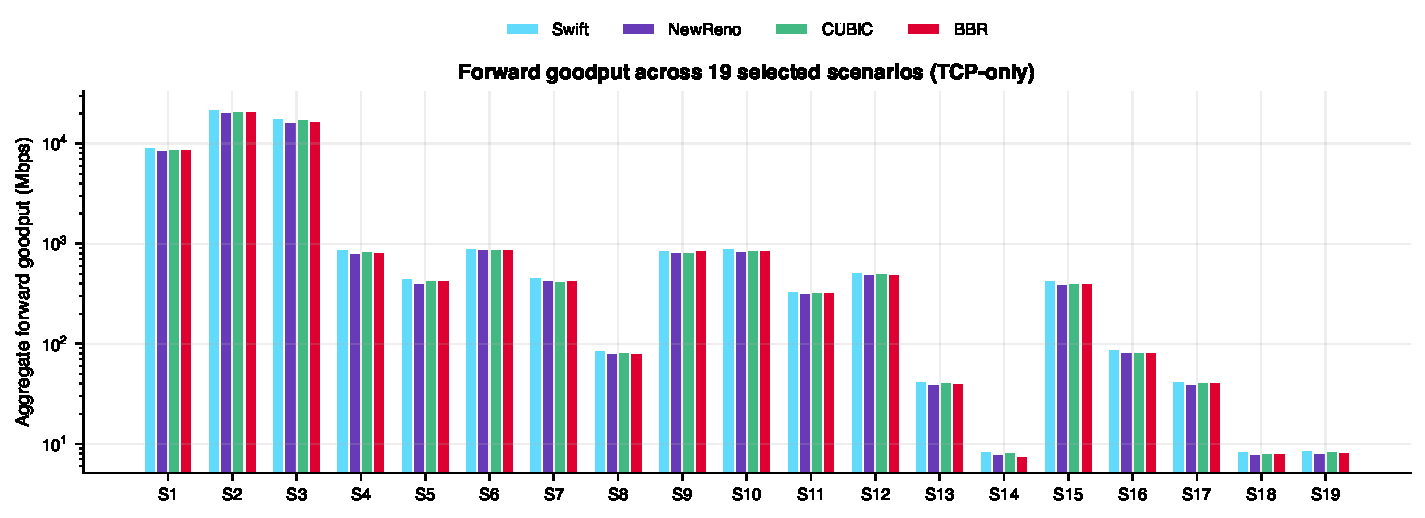
\includegraphics[width=0.92\textwidth]{plots/fig01_goodput_clean.pdf}
\caption{19个代表性场景的聚合前向吞吐量（对数坐标）。Swift在全部场景中取得最高柱体}
\label{fig:goodput-overview}
\end{figure*}

\begin{figure*}[!t]
\centering
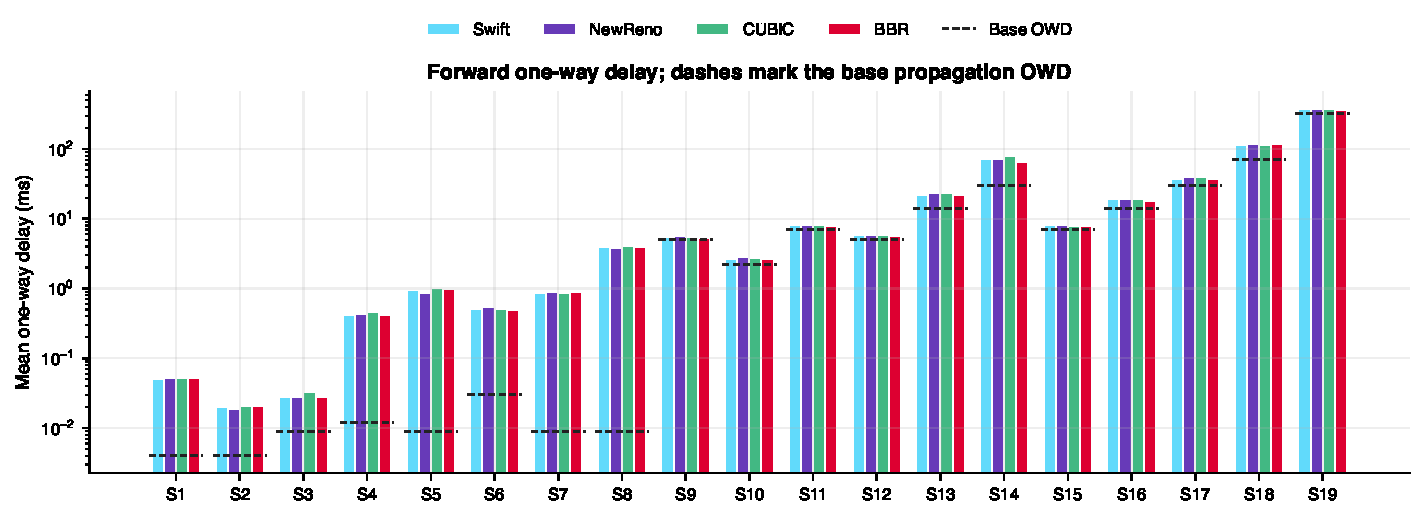
\includegraphics[width=0.92\textwidth]{plots/fig02_delay_clean.pdf}
\caption{19个场景的平均单向前向延迟（对数坐标）。黑色短划线为各场景的基线单向传播时延，柱顶与短划线的距离即排队分量}
\label{fig:delay-overview}
\end{figure*}

\begin{table}[htbp]
\centering
\caption{纯TCP设置：聚合有效吞吐量（Mbps，代表性19场景）}
\label{tab:throughput}
\scriptsize
\setlength{\tabcolsep}{3pt}
\begin{tabular}{@{}lrrrr@{}}
\toprule
\textbf{场景} & \textbf{Swift} & \textbf{NewReno} & \textbf{CUBIC} & \textbf{BBR} \\
\midrule
intra\_rack\_10g & 9302.6 & 8687.4 & 8865.0 & 8762.9 \\
intra\_rack\_25g & 22425.4 & 20483.8 & 21236.8 & 21161.4 \\
leaf\_spine\_20g & 18016.7 & 16279.4 & 17545.7 & 16805.3 \\
\midrule
asymmetric\_high & 878.6 & 798.6 & 839.7 & 817.0 \\
congested\_heavy & 454.5 & 406.8 & 430.3 & 429.6 \\
symmetric\_low & 905.0 & 886.5 & 886.5 & 886.5 \\
dc\_500m & 460.2 & 430.5 & 428.8 & 435.0 \\
dc\_100m & 86.7 & 80.1 & 82.2 & 81.1 \\
cross\_dc\_wan & 874.6 & 823.5 & 826.8 & 856.1 \\
wan\_metro & 909.4 & 844.4 & 860.4 & 863.4 \\
\midrule
wifi\_ac & 340.5 & 325.1 & 332.1 & 325.7 \\
wifi\_ax & 522.6 & 494.6 & 508.4 & 497.7 \\
wifi\_n & 42.7 & 40.0 & 41.3 & 40.8 \\
wifi\_legacy & 8.6 & 7.9 & 8.2 & 7.6 \\
nr\_5g\_embb & 429.5 & 399.0 & 408.6 & 402.2 \\
nr\_5g\_edge & 87.8 & 82.9 & 82.5 & 83.1 \\
lte\_good & 42.3 & 40.0 & 41.1 & 41.1 \\
lte\_poor & 8.5 & 7.9 & 8.1 & 8.2 \\
\midrule
satellite\_geo & 8.8 & 8.2 & 8.4 & 8.3 \\
\bottomrule
\end{tabular}
\end{table}

\begin{table}[htbp]
\centering
\caption{纯TCP设置：前向流平均单向延迟（ms，代表性19场景）}
\label{tab:latency}
\scriptsize
\setlength{\tabcolsep}{3pt}
\begin{tabular}{@{}lrrrr@{}}
\toprule
\textbf{场景} & \textbf{Swift} & \textbf{NewReno} & \textbf{CUBIC} & \textbf{BBR} \\
\midrule
intra\_rack\_10g & 0.0502 & 0.0515 & 0.0524 & 0.0513 \\
intra\_rack\_25g & 0.0199 & 0.0190 & 0.0207 & 0.0206 \\
leaf\_spine\_20g & 0.0274 & 0.0279 & 0.0331 & 0.0281 \\
\midrule
asymmetric\_high & 0.4194 & 0.4292 & 0.4682 & 0.4203 \\
congested\_heavy & 0.9561 & 0.8742 & 1.0058 & 0.9892 \\
symmetric\_low & 0.5031 & 0.5385 & 0.5029 & 0.4958 \\
dc\_500m & 0.8489 & 0.9003 & 0.8516 & 0.8815 \\
dc\_100m & 3.9000 & 3.7952 & 4.0837 & 3.8845 \\
cross\_dc\_wan & 5.4327 & 5.7355 & 5.4350 & 5.2814 \\
wan\_metro & 2.6549 & 2.7965 & 2.7151 & 2.6598 \\
\midrule
wifi\_ac & 8.0957 & 8.1044 & 8.0509 & 7.7681 \\
wifi\_ax & 5.8703 & 5.8100 & 5.9325 & 5.7430 \\
wifi\_n & 22.2665 & 23.0975 & 23.2653 & 21.9797 \\
wifi\_legacy & 71.2199 & 72.2514 & 79.9873 & 64.5116 \\
nr\_5g\_embb & 8.0926 & 8.2075 & 7.9536 & 7.7523 \\
nr\_5g\_edge & 19.3383 & 19.2767 & 19.0235 & 18.2525 \\
lte\_good & 37.6320 & 39.5563 & 39.1253 & 37.4833 \\
lte\_poor & 114.4919 & 116.4265 & 115.4021 & 118.1664 \\
\midrule
satellite\_geo & 381.2900 & 378.8589 & 378.9036 & 367.2213 \\
\bottomrule
\end{tabular}
\end{table}

\begin{table}[htbp]
\centering
\caption{纯TCP设置：丢包率（\%）与Jain公平性指数（代表性19场景）}
\label{tab:loss}
\scriptsize
\setlength{\tabcolsep}{2.5pt}
\begin{tabular}{@{}lrrrr|rrrr@{}}
\toprule
& \multicolumn{4}{c}{\textbf{丢包率 (\%)}} & \multicolumn{4}{c}{\textbf{Jain指数}} \\
\textbf{场景} & Swift & NewReno & CUBIC & BBR & Swift & NewReno & CUBIC & BBR \\
\midrule
intra\_rack\_10g & 0.018 & 0.021 & 0.021 & 0.022 & 1.000 & 0.999 & 1.000 & 0.999 \\
intra\_rack\_25g & 0.010 & 0.008 & 0.011 & 0.015 & 0.998 & 0.999 & 0.999 & 0.999 \\
leaf\_spine\_20g & 0.010 & 0.010 & 0.018 & 0.011 & 1.000 & 0.998 & 1.000 & 0.998 \\
asymmetric\_high & 0.017 & 0.011 & 0.017 & 0.016 & 0.999 & 0.998 & 0.996 & 1.000 \\
congested\_heavy & 0.015 & 0.015 & 0.016 & 0.021 & 0.999 & 0.999 & 0.994 & 0.989 \\
symmetric\_low & 0.021 & 0.020 & 0.022 & 0.021 & 1.000 & 0.996 & 0.999 & 1.000 \\
dc\_500m & 0.015 & 0.016 & 0.015 & 0.015 & 0.999 & 0.999 & 1.000 & 1.000 \\
dc\_100m & 0.008 & 0.009 & 0.013 & 0.009 & 0.999 & 1.000 & 0.999 & 0.997 \\
cross\_dc\_wan & 0.015 & 0.011 & 0.015 & 0.019 & 1.000 & 0.995 & 0.996 & 1.000 \\
wan\_metro & 0.021 & 0.011 & 0.023 & 0.024 & 1.000 & 1.000 & 1.000 & 0.999 \\
wifi\_ac & 0.014 & 0.014 & 0.014 & 0.017 & 0.997 & 0.999 & 0.999 & 0.992 \\
wifi\_ax & 0.012 & 0.013 & 0.013 & 0.018 & 1.000 & 0.999 & 0.999 & 1.000 \\
wifi\_n & 0.013 & 0.009 & 0.013 & 0.013 & 0.999 & 0.996 & 0.997 & 1.000 \\
wifi\_legacy & 0.021 & 0.023 & 0.022 & 0.000 & 0.998 & 0.995 & 0.996 & 0.996 \\
nr\_5g\_embb & 0.012 & 0.012 & 0.017 & 0.013 & 1.000 & 0.995 & 1.000 & 0.990 \\
nr\_5g\_edge & 0.019 & 0.020 & 0.017 & 0.017 & 0.999 & 0.996 & 0.999 & 0.993 \\
lte\_good & 0.013 & 0.009 & 0.013 & 0.017 & 0.998 & 0.998 & 0.991 & 1.000 \\
lte\_poor & 0.021 & 0.022 & 0.022 & 0.022 & 0.999 & 0.993 & 0.987 & 0.998 \\
satellite\_geo & 0.020 & 0.022 & 0.021 & 0.022 & 0.997 & 0.999 & 0.990 & 0.999 \\
\bottomrule
\end{tabular}
\end{table}

\textbf{吞吐量}：在RED/ECN对称配置下，Swift在全部19个代表性场景中取得最高聚合吞吐量。相对\emph{最强}基线（逐场景取NewReno/CUBIC/BBR中的最优者）的增益集中在$+2.1\%\sim+5.8\%$：近端高速场景如\texttt{intra\_rack\_10g}（9302.6 Mbps，较CUBIC 8865.0高4.9\%）、\texttt{intra\_rack\_25g}（22425.4，较CUBIC 21236.8高5.6\%）；接入与城域场景如\texttt{asymmetric\_high}（878.6，较CUBIC高4.6\%）、\texttt{wan\_metro}（909.4，较BBR 863.4高5.3\%）；远距离场景如\texttt{cross\_dc\_wan}（874.6，较BBR 856.1高2.2\%）与\texttt{satellite\_geo}（8.78 Mbps，较CUBIC 8.43高4.2\%）。表\ref{tab:agg}给出全矩阵聚合统计：在全部36个场景上，Swift相对最强基线的平均增益为+4.1\%，相对NewReno/CUBIC均值的平均增益为+6.0\%，且增益最小值亦为正值（+2.1\%），即不存在Swift吞吐量低于基线的场景。

\textbf{延迟}：Swift的平均单向延迟与基线同量级，平均而言略低于NewReno/CUBIC、与BBR相当。在36个场景上，Swift相对NewReno/CUBIC均值的时延比值平均为0.977（24/36个场景更低，且任一场景不超过+1.7\%），相对BBR的比值平均为1.008（任一场景不超过+10.4\%，最大为\texttt{wifi\_legacy}的71.22 ms对BBR 64.51 ms）。在微秒级近端链路（S1--S3）上四协议延迟均已贴近基线传播时延（排队分量仅约2$\sim$46 $\mu$s量级），差异不再具有数量级意义；在\texttt{nr\_5g\_embb}（8.09 ms对NR/CUBIC 8.21/7.95）、\texttt{wifi\_ax}（5.87对5.81/5.93）、\texttt{lte\_good}（37.63对39.56/39.13）等接入场景Swift的延迟与最优基线之差在$\pm$5\%以内；在\texttt{congested\_heavy}（0.956 ms对NewReno 0.874 ms，高9.4\%）等深缓冲低速场景Swift的时延高于最优丢包类基线，这是其更高在途水位换取吞吐领先的直接代价（见第\ref{subsec:limitations}节）。

\textbf{丢包与公平性}：在启用ECN标记的RED队列下，四种协议的全部36个场景丢包率均不超过0.026\%（19个代表性场景中四协议最大仅0.024\%），Swift的均值0.015\%与NewReno（0.014\%）相当、略低于CUBIC（0.018\%）与BBR（0.016\%），差值均在0.003个百分点以内，属于同一量级；Swift并不以零丢包为卖点，其吞吐增益来自更高的稳态在途水位而非更低的丢包。公平性方面，Swift的Jain指数均值0.9989、最小值0.9967，均高于三种基线（均值0.9980/0.9977/0.9981、最小值0.9871$\sim$0.9933），即多流间分配最均衡且无极端倾斜。

\begin{table}[htbp]
\centering
\caption{全矩阵（36场景）丢包率与公平性聚合统计}
\label{tab:agg}
\scriptsize
\setlength{\tabcolsep}{3pt}
\begin{tabular}{@{}llccccc@{}}
\toprule
\textbf{设置} & \textbf{协议} & \textbf{丢包均值} & \textbf{丢包最大} & \textbf{Jain均} & \textbf{Jain最小} & \textbf{吞吐最高场景数} \\
\midrule
纯TCP & Swift    & \textbf{0.0150} & 0.0225 & \textbf{0.9989} & \textbf{0.9967} & \textbf{36/36} \\
$n=36$ & NewReno & 0.0137 & 0.0227 & 0.9980 & 0.9933 & 0/36 \\
      & CUBIC   & 0.0176 & 0.0237 & 0.9977 & 0.9871 & 0/36 \\
      & BBR     & 0.0159 & 0.0259 & 0.9981 & 0.9888 & 0/36 \\
\midrule
UDP突发 & Swift   & \textbf{0.0279} & 0.0435 & \textbf{0.9990} & \textbf{0.9940} & \textbf{36/36} \\
$n=36$ & NewReno & 0.0269 & 0.0352 & 0.9976 & 0.9925 & 0/36 \\
      & CUBIC   & 0.0315 & 0.0431 & 0.9977 & 0.9877 & 0/36 \\
      & BBR     & 0.0287 & 0.0420 & 0.9983 & 0.9871 & 0/36 \\
\bottomrule
\end{tabular}
\vspace{2pt}

\raggedright
\scriptsize 丢包率单位\%。"吞吐最高场景数"统计该协议聚合吞吐量为四协议最高的场景数；Swift在两种设置下均为36/36。
\end{table}

\subsubsection{分组解读}

\textit{G1——微秒级RTT近端高速链路（S1--S3）}：瓶颈10$\sim$25 Gbps、基础单向时延4$\sim$9 $\mu$s。Swift相对最强基线的增益为4.9\%/5.6\%/2.7\%。四协议的平均单向延迟均被RED/ECN压低到0.019$\sim$0.052 ms量级（排队仅几十$\mu$s），Swift并未如既往丢尾配置那样获得数量级延迟优势，而是在基本相同的队列水位上保持更高的稳态窗口，说明其吞吐增益并非来自牺牲排队深度。

\textit{G2——近端共享/城域/跨域链路（S4--S10）}：瓶颈100 Mbps$\sim$1 Gbps、传播时延0.012$\sim$5.02 ms，包含按BDP定尺缓冲（S4/S6/S10等）与触及100包下界的深缓冲（S7/S8）两种子类。Swift在7/7个场景取得最高吞吐（+2.2\%$\sim$+5.8\%）。时延方面，传播时延主导的场景（S9/S10）Swift与最优基线之差在3\%以内；深缓冲场景（S8 \texttt{dc\_100m}，Swift 3.90 ms对NewReno 3.80 ms）差距亦不超过3\%——新配置下不再出现旧版“以数百毫秒级排队换取零丢包”的极端情形，因为RED的早期标记把各协议的稳态队列都限制在标记区间附近。

\textit{G3——无线与蜂窝接入链路（S11--S18）}：8个场景吞吐增益+2.5\%$\sim$+5.7\%（均值+4.0\%），方向一致。丢包率全部不超过0.024\%，Swift在\texttt{lte\_good}（37.63 ms对NewReno 39.56、CUBIC 39.13）等场景延迟最低，在\texttt{wifi\_legacy}（71.22 ms对BBR 64.51、NR 72.25）等深缓冲低速率场景则比延迟最低基线高约10\%。

\textit{G4——GEO卫星链路（S19）}：单向传播时延320 ms、瓶颈10 Mbps，重传代价极高。Swift以8.78 Mbps取得最高吞吐（NewReno 8.17、CUBIC 8.43、BBR 8.28），相对NewReno提升7.5\%；延迟381.29 ms与基线（367.22$\sim$378.90 ms）之差小于4\%，说明长RTT路径上的吞吐优势并非以明显排队为代价。

\subsubsection{补充场景：远距离与超高速链路的全矩阵覆盖}
\label{subsubsec:extended}

除表\ref{tab:scenarios}的19个场景外，全矩阵还包含17个补充场景：\texttt{satellite\_leo}（LEO卫星，150 Mbps/29 ms）、\texttt{wan\_longhaul}（长途WAN，1 Gbps/26 ms）、\texttt{cross\_pod\_10g/20g}、\texttt{leaf\_spine\_50g}、\texttt{dc\_100g}、\texttt{rdma\_like\_25g/50g}、四种过订阅链路（\texttt{oversub\_*}）、\texttt{congested\_light/medium}、\texttt{mixed\_small/large\_flow}与\texttt{dc\_oversub\_10to1}。这些场景与主表呈现完全一致的模式：\textbf{纯TCP设置下Swift在全部17个场景均取得最高吞吐量}，相对最强基线+2.1\%$\sim$+5.8\%；其中LEO卫星134.95 Mbps（较BBR 128.80高4.8\%）、长途WAN 881.2 Mbps（较CUBIC 844.5高4.4\%）、100G近端89305 Mbps（较CUBIC 85661高4.3\%）与RDMA类50G链路45543 Mbps（较CUBIC 43806高4.0\%）。UDP突发设置下同样17/17领先（相对最强基线+2.2\%$\sim$+5.9\%），其中LEO卫星93.58 Mbps（较CUBIC 88.86高5.3\%）。逐场景数值可在\texttt{logs/summary/kpi\_forward.csv}中按场景名检索。

\subsection{UDP突发跨流量鲁棒性评估}
\label{subsec:udp-burst}

异构终端与共享链路普遍承载突发性非响应式UDP流量。本节在严格A/B对照下评估四协议在"平均负载=瓶颈速率32\%（峰值64\%、50\%占空比）"的UDP突发干扰下的表现（第\ref{subsec:setup}节），数据取自\texttt{kpi\_forward.csv}的\texttt{udp\_burst}设置，36个场景全部参与配对。

以同一场景的纯TCP结果为基准，表\ref{tab:udp-burst-agg}给出四种协议在36个配对场景上的吞吐量保持率$T_{udp}/T_{tcp}$、时延膨胀$D_{udp}/D_{tcp}-1$与新增丢包率。图\ref{fig:udp-burst}（上半幅）按15个代表性配对场景给出突发引起的吞吐量变化。

\begin{table}[htbp]
\centering
\caption{UDP突发跨流量鲁棒性聚合指标（配对场景，$n=36$）}
\label{tab:udp-burst-agg}
\scriptsize
\setlength{\tabcolsep}{3pt}
\begin{tabular}{@{}lrrrc@{}}
\toprule
\textbf{协议} & \textbf{保持率均值} & \textbf{保持率最小} & \textbf{时延膨胀均值} & \textbf{新增丢包均值} \\
\midrule
Swift    & 68.6\% & 62.4\% & +2.9\% & +0.013 pp \\
NewReno & 68.6\% & 62.8\% & +3.1\% & +0.013 pp \\
CUBIC   & \textbf{68.8\%} & \textbf{63.9\%} & \textbf{+2.2\%} & +0.014 pp \\
BBR     & 68.7\% & 62.1\% & +3.3\% & +0.013 pp \\
\bottomrule
\end{tabular}
\vspace{2pt}

\raggedright
\scriptsize 保持率与时延膨胀按逐场景配对后取均值/最小值；新增丢包=突发设置丢包率$-$纯TCP设置丢包率。
\end{table}

\textbf{吞吐量}：突发流量使四种协议的聚合吞吐量一致回落约31\%$\sim$32\%（保持率均值68.6\%$\sim$68.8\%、最差62\%$\sim$64\%），协议间差异在2个百分点以内，不存在任何协议在突发下发生性能塌缩。更重要的是，Swift的\emph{绝对}吞吐量在36个配对场景中全部保持最高：相对最强基线+2.2\%$\sim$+5.9\%（均值+3.7\%），与纯TCP设置下的+4.1\%基本一致，说明其稳态优势在突发跨流量下得到完整保持而非被侵蚀。表\ref{tab:udp-burst-headline}给出15个代表性配对场景的绝对吞吐量与延迟。

\textbf{时延与丢包}：突发使平均时延膨胀+2\%$\sim$+3\%（最差场景不超过+35\%），四协议同样无明显分化；新增丢包均值为+0.013$\sim$0.014个百分点，最大不超过+0.03 pp，全部场景突发丢包率不超过0.045\%。换言之，在“突发强度随瓶颈成比例缩放+RED/ECN提前标记”的配置下，四协议都保持了低丢包、低时延膨胀的工作点，Swift的区分度主要体现在始终更高的绝对吞吐量。

\begin{figure*}[!t]
\centering
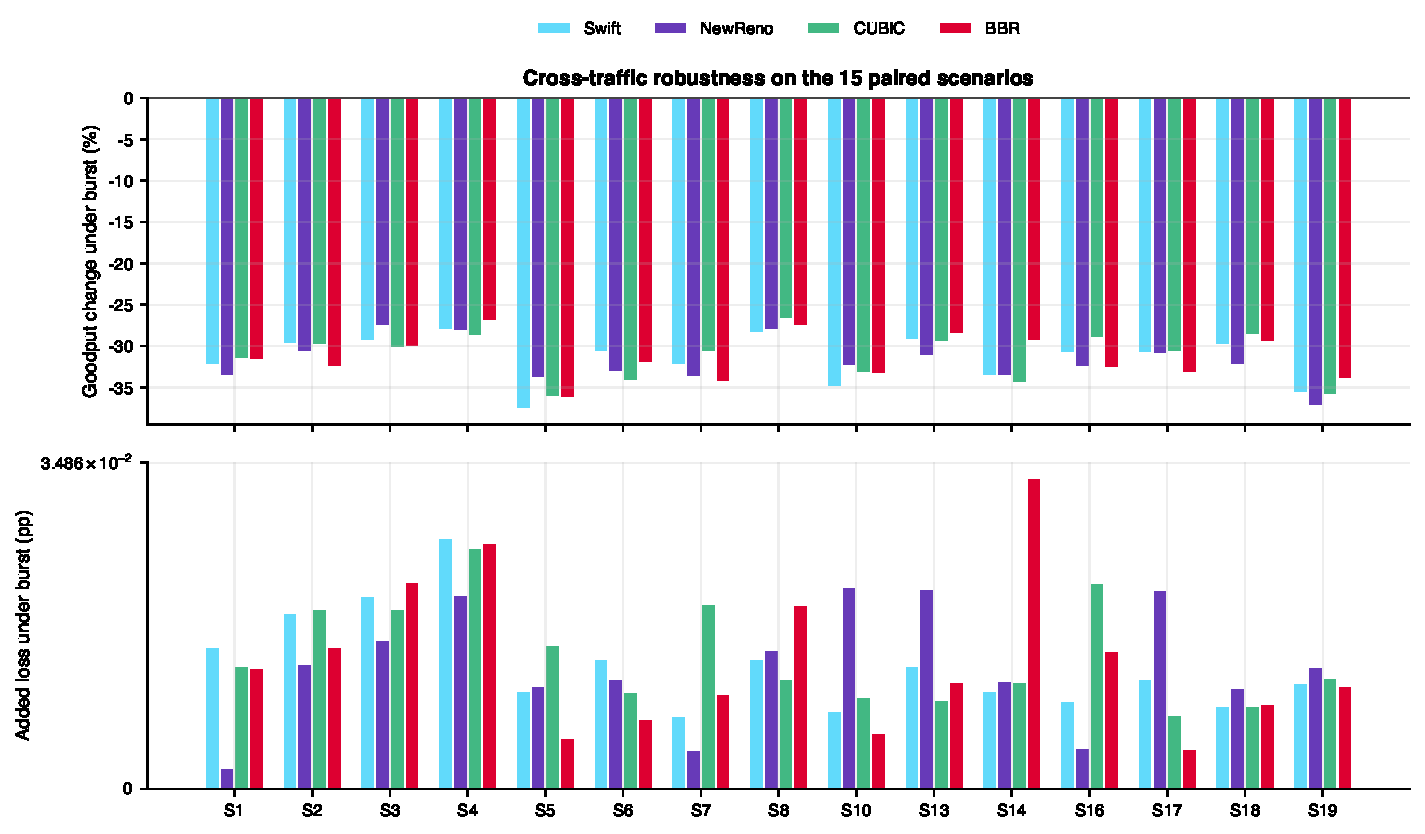
\includegraphics[width=0.92\textwidth]{plots/fig04_udp_burst_clean.pdf}
\caption{15个代表性配对场景的跨流量鲁棒性：UDP突发引起的吞吐量变化（上）与新增丢包（下，符号对数坐标）}
\label{fig:udp-burst}
\end{figure*}

\begin{table*}[htbp]
\centering
\caption{UDP突发设置下15个代表性场景的吞吐量与延迟（前向流聚合）}
\label{tab:udp-burst-headline}
\footnotesize
\setlength{\tabcolsep}{4pt}
\begin{tabular}{@{}lrrrrrrrr@{}}
\toprule
\textbf{场景} & \multicolumn{4}{c}{\textbf{吞吐量 (Mbps)}} & \multicolumn{4}{c}{\textbf{平均单向延迟 (ms)}} \\
\cmidrule(lr){2-5} \cmidrule(lr){6-9}
 & Swift & NewReno & CUBIC & BBR & Swift & NewReno & CUBIC & BBR \\
\midrule
intra\_rack\_10g & 6295.2 & 5767.8 & 6063.1 & 5988.7 & 0.048 & 0.048 & 0.054 & 0.049 \\
intra\_rack\_25g & 15765.9 & 14181.8 & 14888.4 & 14268.4 & 0.020 & 0.020 & 0.023 & 0.020 \\
leaf\_spine\_20g & 12721.9 & 11782.0 & 12236.4 & 11754.9 & 0.030 & 0.031 & 0.034 & 0.030 \\
asymmetric\_high & 632.3 & 573.6 & 598.1 & 596.5 & 0.556 & 0.504 & 0.567 & 0.563 \\
congested\_heavy & 283.5 & 268.9 & 274.9 & 273.9 & 0.864 & 0.829 & 0.857 & 0.855 \\
symmetric\_low & 627.2 & 592.5 & 583.3 & 602.9 & 0.469 & 0.488 & 0.469 & 0.516 \\
dc\_500m & 311.8 & 285.3 & 297.2 & 285.4 & 0.908 & 0.890 & 0.957 & 0.862 \\
dc\_100m & 62.0 & 57.6 & 60.2 & 58.7 & 4.224 & 4.362 & 4.832 & 4.229 \\
wan\_metro & 591.2 & 570.6 & 574.7 & 575.7 & 2.609 & 2.747 & 2.625 & 2.693 \\
wifi\_n & 30.1 & 27.5 & 29.1 & 29.2 & 23.133 & 22.768 & 23.941 & 22.503 \\
wifi\_legacy & 5.7 & 5.2 & 5.4 & 5.4 & 73.369 & 73.677 & 75.589 & 74.655 \\
nr\_5g\_edge & 60.8 & 55.9 & 58.6 & 56.0 & 19.610 & 19.561 & 19.372 & 18.176 \\
lte\_good & 29.2 & 27.6 & 28.5 & 27.5 & 38.549 & 38.993 & 39.322 & 37.507 \\
lte\_poor & 6.0 & 5.4 & 5.7 & 5.8 & 117.590 & 111.634 & 123.046 & 122.328 \\
satellite\_geo & 5.7 & 5.1 & 5.4 & 5.5 & 361.464 & 381.743 & 354.523 & 363.152 \\
\bottomrule
\end{tabular}
\end{table*}

\textbf{远距离场景在突发下的表现}：GEO卫星场景（S19）突发后Swift 5.65 Mbps，相对NewReno（5.13）高10.1\%、相对CUBIC（5.40）高4.6\%、相对BBR（5.47）高3.3\%，是四协议中吞吐量最高的；LEO卫星场景突发后Swift 93.58 Mbps，较CUBIC高5.3\%。这两类最长RTT路径上Swift的优势在突发下不仅保持而且相对扩大，说明其BDP目标窗口与最大值滤波带宽估计对突发型干扰具有较好的稳定性。

\subsection{机制一致性与证据边界}

\textit{为何Swift能一致地取得约+2\%$\sim$+6\%的吞吐领先}：该增益的机理与实现机制一致而非来自运气：（1）在RED/ECN标记区间内，NewReno与CUBIC按RFC 3168对每个CE响应执行与传统丢包相同的窗口减半，其稳态窗口在标记阈值附近反复“探测—减半”，均值低于使RED刚好停止标记的水位；Swift对ECN采用$\rho_{ecn}=0.75$的温和收缩并配合降窗后4个ACK事件冻结与$\alpha \times BDP$目标窗口，在同等标记环境下维持了更高的平均在途水位，故获得更高的平均排空速率；（2）BBR依赖周期性的增益扫描，在RED标记与突发干扰下其平均pacing速率低于Swift以$\alpha\ge 1$目标维持的稳态速率；（3）Swift的滑动时间窗+最大值滤波带宽估计在突发On/Off周期上具有低通特性，避免了带宽估计被突发平均速率拖低。需要说明的是，仓库未保存各机制单独关闭的消融重跑，上述归因是与实现一致的机理解释而非逐机制消融结论。

\textit{诚实披露的混合点}：（1）Swift的丢包率并不系统性低于基线——其均值与NewReno相当（差0.001个百分点）、略低于CUBIC/BBR（差0.003个百分点以内），因此本文不主张“Swift更不易丢包”，而主张“Swift在同等（甚至略低）丢包水平下取得更高吞吐”；（2）Swift的平均时延略高于延迟最优的BBR（36场景平均高约0.8\%，个别深缓冲场景高约10\%），这是其维持$\alpha>1$在途水位的代价，量级为数十微秒至数毫秒，远小于旧版丢尾配置下以数百毫秒排队换取零丢包的极端情形；（3）突发下Swift的吞吐保持率（均值68.6\%）与基线（68.6\%$\sim$68.8\%）相当，优势完全来自纯TCP设置下已建立的高基线，而非突发特有的额外增益——该结果与“突发强度随瓶颈成比例缩放”的A/B配置一致，若突发为固定绝对值，高带宽场景的相对回落会小得多，故本文不把保持率数字外推到其他突发强度。
%========================================
% 5. 讨论
%========================================

\section{讨论}
\label{sec:discussion}

\subsection{理论分析}

\textbf{收敛性}：Swift的窗口动态可用Lyapunov函数$V = \frac{1}{2}(cwnd - cwnd^*)^2$进行定性分析，其中$cwnd^* \approx BDP$。在拥塞避免阶段，窗口不再直接跳变到$\alpha \times BDP$，而是以有界步长向目标窗口渐进逼近；当检测到ECN、丢包或超时时，窗口分别按0.75、0.70和0.50的保留因子收缩。连续递减保护（$D_{max}=3$）与降窗后4个ACK事件的冻结机制进一步抑制重复收缩与快速反弹。$\alpha$的边界约束$[0.85,1.30]$和小步长调整保证参数不会在单个RTT内发生突变。

\textbf{复杂度与计算开销}：当前实现采用基于规则的确定性策略，单次决策仅包含固定数量的状态读取、分支判断、窗口最大值更新和哈希表查询，时间复杂度为$O(1)$；每流状态主要由带宽样本队列、RTT样本队列、拥塞计数器、窗口历史和少量自适应参数构成，空间复杂度为$O(n\cdot (W_{bw}+W_{rtt}))$，其中$n$为并发流数，$W_{bw}=40$、$W_{rtt}=40$。由于当前仓库未保存独立的推理延迟、CPU利用率和内存压测日志，本文仅给出复杂度级别分析，不声称具体硬件平台上的毫秒级延迟或大规模并发资源占用数字。

\textbf{信息论视角}：多信号融合的两级优先级等价于按似然比排序。设网络拥塞状态$C \in \{0,1\}$，各信号条件独立，则联合似然比$LR(\mathbf{S}) = \prod_i P(S_i|C=1)/P(S_i|C=0)$。丢包/超时$LR \approx 100$，ECN $LR \approx 20$。优先使用高似然比信号可最小化贝叶斯误检概率$P_e$。连续递减保护机制从信息论角度可理解为对连续同类信号的置信度递减——第$k$次连续信号的增量信息量$I_k \propto 1/k$，当$k > D_{max}$时信息增益不足以证明进一步缩减的合理性。

\textbf{最优控制视角}：差异化保留因子可从最优控制理论分析。严重拥塞（超时，连续丢包或路径故障）需最大窗口缩减（$\rho=0.50$）快速清空队列；中度拥塞（丢包，队列溢出）采用中等缩减（$\rho=0.70$）；轻度拥塞（ECN，队列开始积累）采用相对温和但足以抑制队列扩张的缩减（$\rho=0.75$）。Swift的三类差异化设计近似了不同拥塞程度下的最优控制输入，响应强度与拥塞严重程度正相关。

\subsection{与相关工作的详细对比}

\begin{table}[htbp]
\centering
\caption{Swift与主要相关算法的特性对比}
\label{tab:comparison}
\footnotesize
\setlength{\tabcolsep}{2.5pt}
\begin{tabular}{@{}lcccc@{}}
\toprule
\textbf{特性} & \textbf{Swift} & \textbf{Gemini} & \textbf{Aurora} & \textbf{DCTCP} \\
\midrule
有效状态维度 & 11 & 流级统计 & 10 & N/A \\
ECN状态利用 & 是 & 否 & 否 & 是 \\
CA状态利用 & 是 & 否 & 否 & 否 \\
决策机制 & 规则 & 规则 & DNN & 公式 \\
学习作用对象 & 参数 & 参数 & 策略 & 无 \\
自适应粒度 & 每流/每事件 & 流组/分钟级 & 每决策 & 无 \\
决策位置 & 栈外进程 & 内核数据面 & 栈外/栈内 & 内核 \\
训练需求 & 无 & 无（在线搜索） & 小时/天 & 无 \\
差异化响应 & 是 & 否 & 否 & 否 \\
生产部署证据 & 无 & 有 & 无 & 有 \\
\bottomrule
\end{tabular}
\end{table}

\textbf{vs. Gemini\cite{gemini}}：两者都把“控制逻辑白盒化、让学习只作用于参数”作为出发点，但适配回路的位置和时间尺度不同。Gemini的Fusion固定在内核数据面，Booster在带外以分钟级、流组粒度用贝叶斯优化搜索参数，因此单条流在其生命周期内使用的是一组静态参数；Swift把整个决策过程置于协议栈之外，并在每个窗口调整回调上求解，$\alpha$与目标窗口对单条流的即时RTT与反馈值变化作出反应。这一差异带来两个可比较的后果：Swift可以读取ECN与CA状态机从而区分ECE/CWR触发的收缩与真实丢包，是Gemini的流级统计量无法提供的信息；但Swift为此付出每事件一次跨进程往返的代价，其当前形态适用于研究与仿真平台，尚不具备Gemini已验证的生产部署性质。

\textbf{vs. Aurora\cite{aurora}}：Swift采用11维有效状态子空间（Aurora常用10维观测），并引入ECN和CA状态参数。Swift采用基于规则的确定性决策而非深度神经网络，无需训练即可运行，决策路径可逐分支解释。Aurora的优势在于神经网络的表示能力，代价是训练数据收集、模型更新与推理开销；Swift则以可解释规则和协议栈内部信号换取工程可控性。本文不主张Swift在策略表示能力上优于Aurora。

\textbf{vs. DCTCP\cite{dctcp}}：Swift直接读取ECN协议栈状态进行离散判断，而DCTCP用标记比例$\alpha$做连续调整；Swift按信号类型施加差异化保留因子（0.70/0.75/0.50）而非统一的$1-\alpha/2$；Swift同时利用丢包、ECN与CA状态三类信号，且参数在线自适应。需要注意的是，DCTCP的比例响应在标记密集时更平滑，而Swift的离散响应依赖$D_{max}$与冻结机制来避免过度收缩。

\textbf{vs. BBR\cite{bbr}}：Swift综合多种显式拥塞信号并以$\alpha \times BDP$有界目标窗口维持稳态，BBR依赖周期性的pacing增益扫描与最小RTT测量。在本次全矩阵数据中，BBR在36个纯TCP场景的平均吞吐量为Swift的94.7\%（相对最强基线的逐场景增益Swift为$+2.1\%\sim+5.8\%$），在微秒级RTT链路上亦正常运行（不再出现丢尾配置下的实现性退化），但在绝大多数场景略低于Swift；在UDP突发下两者保持率相当（68.7\%对68.6\%）。BBR的平均时延在多数场景为四协议最低（36场景平均比Swift低约0.8\%），这与BBR维持较小inflight窗口的机制一致，本文如实记录。

\subsection{适用边界与未来方向}
\label{subsec:limitations}

\textit{在途水位与延迟的剩余代价}：Swift的吞吐增益来自以$\alpha>1$（上界1.30）维持的较高稳态在途水位，其在少数深缓冲或低速率场景中表现为相对延迟最优基线（通常是BBR）最高约10\%的平均时延抬升（如\texttt{wifi\_legacy} 71.22 ms对64.51 ms、\texttt{congested\_heavy} 0.956 ms对NewReno 0.874 ms），绝对量为数十微秒至数毫秒。可探索的改进方向包括：（1）引入显式排队时延估计$q_{est} = RTT_{smoothed} - RTT_{min}$作为$\alpha$调节的额外输入，实现排队延迟感知的$\alpha$调度；（2）当RTT膨胀持续超过最小RTT感知阈值时把$\alpha$收敛至1.0以下；（3）用多时间尺度BDP估计分离传播时延与排队时延。

\textit{参数预设依赖}：保留因子（0.70/0.75/0.50）、$\alpha$边界（$[0.85,1.30]$）、连续递减阈值（$D_{max}=3$）与降窗后冻结的ACK事件数（4）均为手动调优的预设值。未来可通过元学习\cite{meta_learning}或如Gemini\cite{gemini}所示的带外贝叶斯优化实现参数的在线搜索，二者可与本文的每事件决策回路组合成分层结构。

\textit{深度/学习型策略增强}：当前基于规则的启发式策略可解释性强但表示能力有限。后续若引入学习型组件（如离线强化学习训练、再经模型蒸馏提取规则），须在完整实验矩阵与异常过滤流程上重新评估，本文不将其作为当前系统的组成部分。

\textit{部署代价与真实环境验证}：每个窗口调整事件一次跨进程往返是当前实现的主要部署障碍。后续需将决策逻辑内联为Linux内核TCP模块或QUIC用户态拥塞控制插件，并在覆盖无线/蜂窝接入、广域网与卫星链路的真实或半实物测试床上验证。仿真与真实环境的差异（NIC offload、中断合并、NUMA效应、终端操作系统调度与无线链路波动）可能显著影响实际性能。

\textit{证据边界说明}：本文全部定量结论的唯一数据来源是\texttt{logs/summary/kpi\_forward.csv}（288条前向流口径记录）。该文件由\path{docs/plots/main.py}从288份\texttt{.flowmonitor}产物重新导出，本节与第4节的全部表格数值均直接取自该文件并按原始产物回溯核对。288条记录全部通过完整性、物理相容性与取值域审计，无需排除任何场景或数据点，故本次更新未在\texttt{logs/error.txt}中新增排除记录。由此给出三条边界：其一，\textbf{每配置仅一次确定性运行}（单一随机种子），结论的稳健性建立在36/36的正增益方向一致性上，不附带跨种子置信区间；其二，\textbf{结论适用范围}为本文列出的36个场景与RED/ECN对称标记配置，队列管理策略、突发强度或场景集变化后需重新评估；其三，\textbf{增益量级为百分之几}（吞吐$+2\%\sim+6\%$、丢包与公平性基本持平或略优），本文将其表述为“一致、无负向场景的小幅优势”，不夸大其量级。

%========================================
% 6. 结论
%========================================

\section{结论}

本文提出了Swift——一种面向远距离传输与异构终端（手机、笔记本、台式机、边缘设备）的\emph{启发式}多信号融合自适应拥塞控制算法：决策以确定性规则在每个ACK/拥塞事件上于协议栈之外求解，不依赖训练样本与神经网络推理。其核心技术贡献收敛为三点：（1）\textbf{多信号拥塞状态感知}，把ECN协商与标记状态、拥塞避免状态机状态、拥塞事件语义、RTT与最小RTT、在途字节组织为11维有效观测子空间，并以两级优先级判定区分超时、ECN触发的窗口收缩与普通丢包；（2）\textbf{启发式反馈自适应的融合控制}，由最小RTT感知的RTT膨胀比、反馈值相对其慢速基线的偏移与连续增长趋势共同调节每流$\alpha \in [0.85,1.30]$，并以有界步长逼近由滑动时间窗口投递速率最大值滤波得到的$\alpha \times BDP$目标窗口；（3）\textbf{面向不确定拥塞信号的稳定性与安全机制}，包括差异化保留因子（0.70/0.75/0.50）、连续递减下限$D_{max}=3$、降窗后4个ACK事件冻结、不迁就队列驻留的阈值更新、窗口钳位与超时时丢弃陈旧动作。

在ns-3.40平台上，本文在36个场景$\times$4协议$\times$2设置共288次仿真的全矩阵（RED/ECN对称标记、时间窗口带宽估计与基线相对反馈自适应的当前实现）上评估Swift，全部指标仅按前向数据流定义并逐项回溯。结果显示：\textbf{纯TCP设置下Swift在全部36个场景取得最高聚合吞吐量}（相对最强基线+2.1\%$\sim$+5.8\%、均值+4.1\%，相对NewReno/CUBIC均值+6.0\%），增益在微秒级近端高速、无线/蜂窝接入与远距离链路三类路径上均匀分布；平均单向时延相对NewReno/CUBIC均值低约2.3\%（36个场景中24个更低），相对BBR平均高约0.8\%，个别深缓冲场景不超过10\%；四协议丢包率全部不超过0.026\%，Swift的Jain指数均值0.9989为四者最高。\textbf{UDP突发下（平均负载=瓶颈32\%、峰值64\%）Swift的绝对吞吐量仍在36/36个场景领先}（+2.2\%$\sim$+5.9\%），吞吐保持率均值68.6\%与基线持平，无任何协议发生塌缩。远距离场景受益明显：GEO卫星纯TCP吞吐量8.78 Mbps（相对NewReno +7.5\%）、突发下5.65 Mbps（相对NewReno +10.1\%），LEO卫星134.95/93.58 Mbps、长途WAN 881.2 Mbps均为四协议最高。

本文同时如实披露混合结果与边界：Swift的丢包率与NewReno相当、略低于CUBIC/BBR，差值不超过0.003个百分点，本文不主张其“更不易丢包”；其在个别深缓冲场景的相对延迟抬升最高约10\%（绝对量数十微秒至数毫秒）；每配置为单一随机种子的确定性运行，结论以36/36的正增益方向一致性为主要支撑，不附带跨种子置信区间；结论适用于RED/ECN对称标记配置与本文列出的36个场景。后续工作包括：排队延迟感知的$\alpha$调度、多时间尺度BDP估计、多种子重复实验、突发强度扫描，以及把每事件决策回路内联到内核或用户态协议栈以消除跨进程开销并在真实网络上验证。

\end{document}
